% \chapter*{Anhang}
\addcontentsline{toc}{part}{Anhang}
\setcounter{chapter}{1}

%\section{Quellen im \isi{Korpus} \hai{chrLiJi1}}\label{appendixchrliji1}
% \begin{landscape}
\footnotesize
 \begin{longtable}{l>{\raggedright}p{2cm}>{\raggedright}p{2cm}lllp{2cm}}
	\caption{Quellen im \isi{Korpus} \hai{chrLiJi1}}\label{appendixchrliji1}
\\
\lsptoprule
 Kürzel & Titel & Autor & Jahr & Ort & Typ & Gattung \\ 
\midrule\endfirsthead
Kürzel & Titel & Autor & Jahr & Ort & Typ & Gattung \\ \midrule\endhead
\lspbottomrule\endlastfoot
OF & Die auff den traurigen Ascher-Mittwoch der Juden erfolgte Oster-Freudt  & n.a. & 1711 & Frankfurt a. \,M.& B2 & Pamphlet \\ 
LR & Poëtische Leichen-Rede  & n.a. & 1730 & Prag & B2 & Prosa\-gedicht \\ 
NF & Neue Fabeln und Erzehlungen in gebundener Schreibart  & n.a. & 1749 & Hamburg & B2 & Gedicht \\ 
AO  & Die abgedankten Offiziere & Johann Gottlob d. J. Stephanie & 1770 & Wien & C2 & Drama \\ 
DW  & Der neue Weiberfeind und die schöne Jüdinn. Ein Lustpiel in fünf Aufzügen & Stephanie d. Ältere & 1773 & Wien & C2 & Drama \\ 
AT  & Der adeliche Tagelöhner & F.G. von Nesselrode zu Hugenboett & 1776 & München & C2 & Drama \\ 
FL  & Fausts Leben  & Mahler Müller & 1778 & Mannheim & B2\slash C2 & Drama \\ 
PL  & Das Purschenleben  & Karl Theodor von Traiteur & 1780 & Mannheim & B2 & Drama \\ 
VE & Verbrechen aus Ehrsucht & August Wilhelm Iffland & 1784 & Mannheim & B2 & Drama \\ 
LB & Der Landjunker in Berlin  & Johann Christian Brandes & 1785 & Berlin & B2 & Drama \\ 
AH  & Armuth und Hoffarth  & Johann David Beil & 1789 & Chemnitz & C2 & Drama \\ 
PM  & Der Postmeister  & Christian Friedrich Ferdinand Anselm von Bonin & 1792 & Magdeburg & B2 & Drama \\ 
FE  & Friedrich Ehrenwerth  & E.F.F. & 1794 & Leipzig & B2 & Drama \\ 
BS & Bettelstolz & David Beil & 1798 & Mannheim & C2 & Drama \\ 
EJ  & Ende des 18ten Jahrhunderts  & n.a. & 1799 & n.a. & C2 & Drama \\ 
WA  & Der weibliche Abaelino oder das Maedchen in vielerlen Gestalten  & Georg Ludwig Peter Sievers & 1802 & Magdeburg & B2 & Drama \\ 
NW & Der travestierte Nathan der Weise  & Julius v. Voß & 1804 & Berlin & C2 & Drama \\ 
FS  & Der feindliche Sohn & Christlieb Georg Heinrich Arresto & 1805 & Schwerin & C2 & Drama \\ 
PS  & Der Proceß in Südpreußen  & Julius v. Voß & 1808 & Berlin & C2 & Drama \\ 
JK  & Jakobs Kriegsthaten und Hochzeit  & Karl Borromäus Sessa & 1810 & Breslau & B2 & Drama \\ 
HJ  & Halle und Jerusalem  & Carl Joachim Friedrich Ludwig (Achim) von Arnim & 1811 & Berlin & B2 & Drama \\ 
PF & Pflicht um Pflicht  & Pius Alexander Wolff & 1816 & Augsburg & B2\slash C2 & Drama \\ 
EV & Euer Verkehr & Julius v. Voß & 1817 & Berlin & B2 & Drama \\ 
TH  & Truthähnchen & Hartwig von Hundt-Radowsky & 1820 & Merseburg & B2 & Roman \\ 
MS  & Mustersaal aller deutschen Mund-arten  & Johann Gottlob Radlof & 1822 & Bonn & B2 & Gedicht\slash  Taldmud\-geschichte \\ 
AJ & Das Abenteuer in der Judenschenke  & Louis Angely & 1825 & Berlin & B2 & Drama \\ 
BW  & Die Braunschweiger Wurst  & Christian Gottfried Solbrig & 1826 & Leipzig & B2 & Drama \\ 
GP  & Gedichter, Parabeln unn Schnoukes & Itzig Veitel Stern (Pseud.) & 1831 & Nürnberg & C2 & diverses; \newline vorwiegend\newline episch \\ 
PA  & Der Papier-Markt zu Frankfurt am Main  & Itzig Greif (Pseud.) & 1834 & Frankfurt a.\,M. & C2 & Drama \\ 
PG & Parodiee, Gedichtches unn prousaische Uffsätz' & Christian Heinrich Gilardone & 1835 & Speyer & C2 & diverses; \newline vorwiegend\newline episch \\ 
PP  & Paris in Pommern, oder Die seltsame Testaments=Klausel. & Louis Angely & 1839 & Berlin & B2 & Drama \\ 
IA  & Itzigs Abschied  & Z. Fuuck (Hg.) & 1840 & Erlangen & C2 & Gedicht \\ 
LM  & Das Lied vom Mazes ouder Geld un kah Geld  & Blumenstein, Eissig Hirsch (Pseud.) & 1844 & Würzburg & C2 & Ballade \\ 
AD & Der alte deutsche Degenknopf  & Wilhelm Reinhold & 1846 & Leipzig & B2 & Drama \\ 
LP & Lazarus Polkwitzer von Nikolsburg  & Friedrich Ernst Hopp & 1849 & Brünn & B2\slash C2 & Drama \\ 
AB  & Abenteuer einer Tänzerin  & Pluto (Pseud. Eduard Stiegmann)  & 1850 & Hamburg & B2 & Drama \\ 
FM  & Das Fest des Mercur oder Die Posse im Leben  & C. Goehring & 1852 & Leipzig & B2\slash C2 & Drama \\ 
SH  & Soll und Haben  & Gustav Freytag & 1855 & Kluczbork & B2 & Roman \\ 
DG  & Der Gütsteher  & Reb Gedaljeh Pinkeltroger (pseud.) & 1858 & Wien & C2 & Gedicht\slash Schiller\-parodien \\ 
UT  & Ut mine Stromtid  & Fritz Reuter & 1862 & Stavenhagen & D2 & Auto\-biographie \\ 
MV  & Museum komischer Vorträge für das Haus – und die ganze Welt  & F. E. Moll & 1862 & Berlin & B2\slash C2 & Gedicht \\ 
JD & Ein jüdischer Dienstbote  & Carl Elmar & 1866 & Wien & D2 & Drama \\ 
JP & Jüdische Parodien und Schnurren  & J. Krüger & 1867 & Altona & B2 & Gedichte\slash Schiller\-parodien \\ 
DK  & Das Kreuz  & F. Krone & 1872 & Osterwieck & C2 & Gedicht \\ 
DP & De Peerlotterie!  & Ernst Keller & 1874 & Pyrzyce & C2 & Drama \\ 
BP & Ein Billet von Pauline Lucca  & Robert Karwe & 1875 & Berlin & C2 & Drama \\ 
SV  & Spaßvogel, der jüdische, oder Jocosus hebricosus  & A. L. Berend \& Co & 1890 & Berlin & B2 & diverses; \newline vorwiegend\newline episch \\ 
GW  & 190 gepfefferte jüdische Witze und Anekdoten  & n.a. & 1900 & Berlin\footnote{Inhaltlich eher k.u.k. Raum, daher als n.a. behandelt.} & C2 & Witze \\ 
SS  & Schabbes-Schmus  & Chaim Jossel (pseud.?) & 1907 & Berlin & B2 & diverses; \newline vorwiegend\newline episch \\ 
VD & Vergessene Dichtungen in Frankfurter und Sachsenhäuser Mundart  & M. L. Langenschwarz, J. W. Sauerwein und J. Löhr & 1916 & Frankfurt a.\,M. & C2 & Brief in\newline Reimform \\ 
SB & Die Sünde wider das Blut  & Artur Dinter & 1918 & Hartenstein & B2 & Roman \\ 
LS  & Levi Silberstein in der Klemme  & Peter Kaser & 1925 & Bonn & C2 & Drama \\ 
AK & Als der Krieg zu Ende war & Max Frisch & 1948 & Zürich & D2 & Drama \\ 
\end{longtable}
% \end{landscape}

%  \markboth{Quellen im \isi{Korpus} \hai{chrLiJi1}}{Quellen im \isi{Korpus} \hai{chrLiJi1}}
% 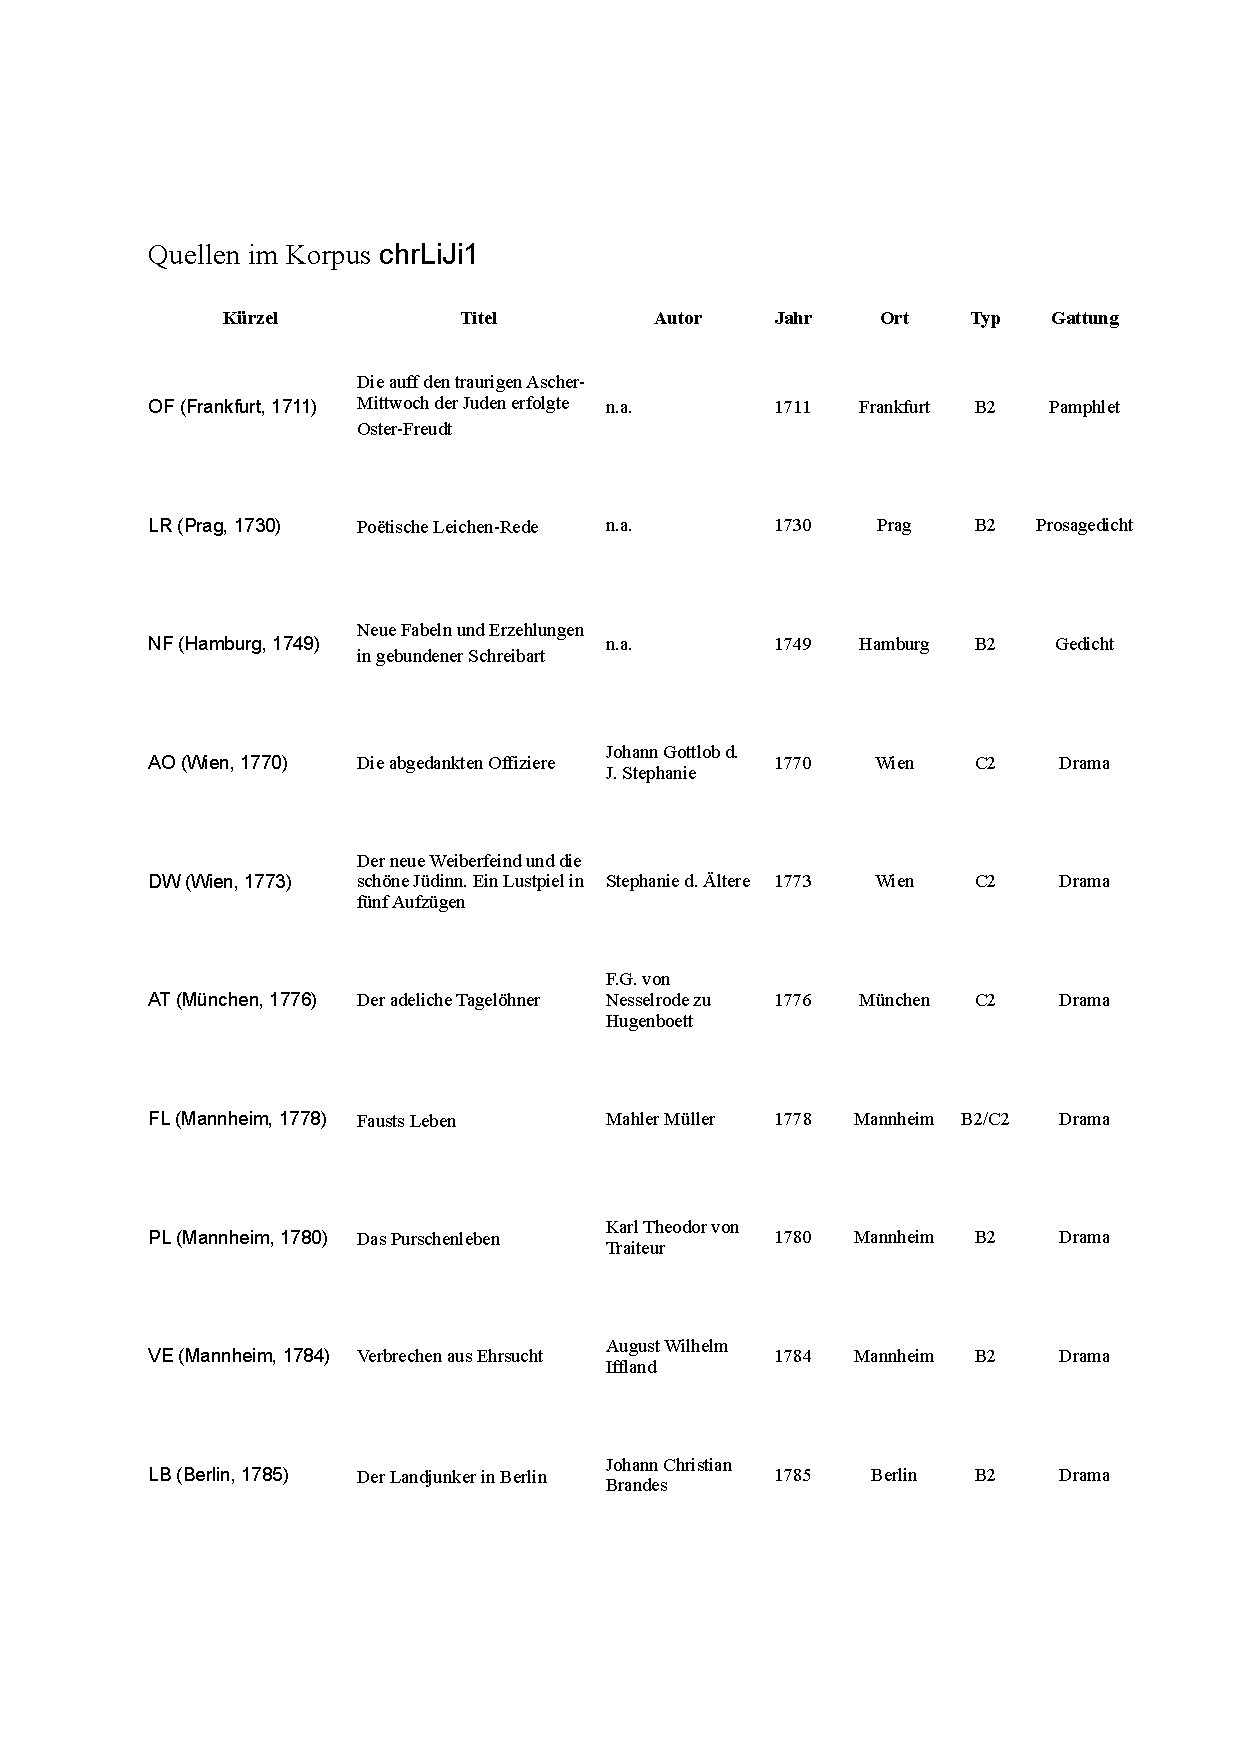
\includepdf[pages=-,pagecommand={\pagestyle{headings}}]{figures/Anhangliji1v.pdf} 

%%%%%%%%%%Quellen im \isi{Korpus} chr\ili{LiJi} ENDE


%%%%Quellen im \isi{Korpus} jüiJi1 ANFANG

\begin{table} 
\caption{Quellen im \isi{Korpus} \hai{jüdLiJi1}}\label{appendixjuedliji1} 
\resizebox{\textwidth}{!}{\begin{tabular}{  l  >{\raggedright}p{4.25cm}  >{\raggedright}p{3cm} r l  }
\lsptoprule
	%Quellen im \isi{Korpus} jüd\ili{LiJi1} &  &  &  &  \\ 
% 	 &  &  &  &  \\ 
	Kürzel & Titel & Autor & \multicolumn{1}{c}{Jahr} & Gattung \\  \midrule
	GuS1 & Schmonzes-Berjonzes  & Nathan Tulpenthal\footnote{Pseudonym\label{AppFnQuellen1}} & ca. 1877 & Sammlung \\ 
	GuS5 & Aufgewärmte Lockschen  & Awrohm Auscher\textsuperscript{\ref{AppFnQuellen1}} & ca. 1877 & Sammlung \\ 
	GuS15 & Schlachmonaus aus Purim  & David Hamanklopper\textsuperscript{\ref{AppFnQuellen1}} & ca. 1867 & Sammlung \\ 
	GuS23 & Was meinen Sie, wie gesund ist das!  & Mortche Omeinsager\textsuperscript{\ref{AppFnQuellen1}} & ca. 1877 & Sammlung \\ 
	GuS10 & Koschere Mezies  & Reb Moser Graggler\textsuperscript{\ref{AppFnQuellen1}} & ca. 1877 & Sammlung \\ 
	PBerlin2 & Waih geschriegen, Mer sain gemacht!!  & Rebbe Jankeff\textsuperscript{\ref{AppFnQuellen1}} & 1848 & Briefform \\ 
	PBreslau & Die jüdische Bürgerwehr  & Siegfried Mehring & n.a. & Pamphlet \\ 
	Palsleben & Herr Richard Wogner, der musikal'sche Struwelpeter %, saane naiste Oper: Trischan Isolldich! %Saane grauße Karophonie ßu Bayreuth un saan forchtbaren Tod 
    & Isaac Moses Hersch & 1876 & Pamphlet \\ 
	PBerlin1 & Gott der Gerechte – Berlin geiht pleite  & Jakob Leibche Tulpenthal  & 1848 & Pamphlet \\ 
	PDebreczen & Jünge Zores ün alte Seferes oder Kosere Tsüwes af trefene Sajles  & Majer Jofeh de Babelebens Enikel  & 1867 & Pamphlet \\ 
\lspbottomrule
\end{tabular}}
\end{table}

\pagebreak
% \markboth{\isi{Frequenz} phonologisch markierter Types im \hai{LiJi1}}{\isi{Frequenz} phonologisch markierter Types im \hai{LiJi1}}
%\section{\isi{Frequenz} phonologisch markierter Types im \hai{LiJi1}}\label{tblFKphon2}

\begin{small}\begin{longtable}{rlp{2cm}p{1.8cm} @{\hspace{.75\tabcolsep}} p{1.75cm} @{\hspace{.75\tabcolsep}} p{1.5cm}}
\caption{\isi{Frequenz} phonologisch markierter Types im \hai{LiJi1}\label{tblFKphon}}\\\lsptoprule Quellen\footnote{Zahl der Korpustexte in denen das Lemma phonologisch manipuliert ist.} & Lemma	 & häufige\newline Manipulation &  \hai{{\FK}} n. Ruoff 1981 \hai{WA}\footnote{Nach Wortart (\hai{WA})} & \hai{{\FK}} n. Ruoff 1981\footnote{Die 
 hier angegebenen \hai{{\FK}}n beruhen ausnahmsweise nicht auf die von Ruoff (1981) vorgenommenen Wortarteneinteilung, sondern sind nach dem Gesamtsample; in diesem Fall ist das Häufigste Lexem \sem{der/dieser} (Häufigkeit = 37536) (vgl. Ruoff 1981:\,514).} 
&\hai{{\FK}} n. \hai{DeReKo} 2012\\\midrule\endfirsthead
\midrule Quellen\footnote{Zahl der Korpustexte in denen das Lemmsmalla phonologisch manipuliert ist.} & Lemma	 & häufige\newline Manipulation &  \hai{{\FK}} n. Ruoff 1981 \hai{WA}\footnote{Nach Wortart (\hai{WA})} & \hai{{\FK}} n. Ruoff 1981\footnote{Die 
 hier angegebenen \hai{{\FK}}n beruhen ausnahmsweise nicht auf die von Ruoff (1981) vorgenommenen Wortarteneinteilung, sondern sind nach dem Gesamtsample; in diesem Fall ist das Häufigste Lexem \sem{der/dieser} (Häufigkeit = 37536) (vgl. Ruoff 1981:\,514).} 
&\hai{{\FK}} n. \hai{DeReKo} 2012\\\midrule\endhead
\lspbottomrule\endlastfoot

52 &	habe(n)\slash hat\footnote{inkl. Hilfsverb.}  &	\textit{hob/hot} & \hai{FK0}\footnote{inkl. Hilfsverb.} & \hai{FK1} & \hai{FK3} \\ 
52 & ein & \textit{a/ä} & \hai{FK2} & \hai{FK2}&  \hai{FK3}  \\
50	& kein	& \textit{kan} & \hai{FK5} & \hai{FK7}& \hai{FK6}\\
46 & groß & \textit{graus/ grois} &\hai{FK1} & \hai{FK6}& \hai{FK6} \\
45 &	auch	 &\textit{aach} & \hai{FK3} & \hai{FK4}& \hai{FK4}\\
42 &	da	& \textit{do/dau} & \hai{FK3} & \hai{FK4}& \hai{FK7} \\
36 & wehe & \textit{waih}  & – & – & \hai{FK26}\\
32& auf &	\textit{uf/af} & \hai{FK2} & \hai{FK4}& \hai{FK4}\\
31 & gehen & \textit{gaihn} & \hai{FK4} & \hai{FK5} & \hai{FK6} \\
30 & schön & \textit{schein} & \hai{FK1} & \hai{FK6}& \hai{FK9} \\
28	& einmal & \textit{amol} & \hai{FK1} & \hai{FK4} & \hai{FK8} \\
24 & sein\footnote{inkl. Hilfsverb.} & \textit{sayn/seyn} &\hai{FK1}\footnote{inkl. Hilfsverb.} & \hai{FK2}\footnote{als Hilfsverb.} & \hai{FK3}\\
24 & kommen & \textit{kummen} & \hai{FK3} & \hai{FK4}& \hai{FK6} \\
20& nicht	 & \textit{nischt} & \hai{FK0} & \hai{FK4}& \hai{FK4} \\
20 & laufen & \textit{laafen} & \hai{FK6} & \hai{FK7}& \hai{FK9} \\
19 &	so& \textit{sau} & \hai{FK1} & \hai{FK6}& \hai{FK5}\\
19 & glauben & \textit{glaaben/ gloiben} & \hai{FK6} & \hai{FK7}& \hai{FK9}\\
19 & sagen & \textit{sogen} & \hai{FK3} & \hai{FK4}& \hai{FK6} \\
18 & Leute  & \textit{Lait} & \hai{FK1} & \hai{FK6}& \hai{FK9}\\
17 & ja & \textit{jau/jo} &  \hai{FK0} & \hai{FK3} & \hai{FK8} \\
17 & mein(e) & \textit{maan(e)} & \hai{FK2} & \hai{FK4}& \hai{FK7} \\
17 & stehen & \textit{steiht}  & \hai{FK6} & \hai{FK7}& \hai{FK6}\\
16 & heißen\footnote{trans. u. intrans.} & \textit{haast} & \hai{FK5}\footnote{trans. u. intrans.} & \hai{FK6} & \hai{FK8}\\
16 & klein & \textit{klaan} & \hai{FK1} & \hai{FK4}& \hai{FK7}\\
15 & was\footnote{inkl. \isi{Relativpartikel}.} & \textit{wos }& \hai{FK4}\footnote{ohne \isi{Relativpartikel}.} & \hai{FK4}\footnote{ohne \isi{Relativpartikel}.}& \hai{FK7}\footnote{ohne \isi{Relativpartikel}.}\\
15 & warum & \textit{worum} & – (z)\footnote{Mit \quein{z} gekennzeichnete Lemmata haben in Ruoff (1981) keine bestimmte Zahl zugewiesen (vgl. Ruoff 1981:\,28).} & – (z) & \hai{FK9} \\
15 & kaufen & \textit{kaafen/ koifen} & \hai{FK6} & \hai{FK7}& \hai{FK10} \\
14 & Tag & \textit{Tog} & \hai{FK1} & \hai{FK5} & \hai{FK7}  \\
13 & mal & \textit{mol} & \hai{FK8} &  \hai{FK8} &\hai{FK10} \\
12 & das & \textit{dos} & \hai{FK0} & \hai{FK2}& \hai{FK0}\slash\hai{FK3} Pron.  \\
12 & tot & \textit{taut/toit} & \hai{FK5} & \hai{FK11}& \hai{FK10}  \\
12 & wissen & \textit{waaß} &  \hai{FK4} & \hai{FK5}& \hai{FK9} \\
11 & es & \textit{‘s} & \hai{FK1} & \hai{FK3}& \hai{FK4} \\
11 & tun & \textit{ton} & \hai{FK4} & \hai{FK7}& \hai{FK8} \\
10 & Auge & \textit{Aage\slash Oige} & \hai{FK6}& \hai{FK10} & \hai{FK9} \\
10 & sie\footnote{Nom.3.Pl., Nom.Sg., Akk.3.Pl., Nom.3.Sg.f., Akk.3.Sg.f.} & \textit{se} & \hai{FK5,4,6,6,6,6} & \hai{FK4,6,7,7,7,9}& \hai{FK5} \\ 
9 & heim & \textit{haam} & – & – & \hai{FK12} \\
9 & hoch & \textit{hauch/hoich} & \hai{FK3}& \hai{FK8}& \hai{FK7} \\
9 & Jahr & \textit{Johr} & \hai{FK0} & \hai{FK5}& \hai{FK5} \\
9 & nur & \textit{nor} & \hai{FK4}& \hai{FK7}& \hai{FK5} \\
9 & oh & \textit{au} & – (z) & – (z)& \hai{FK13} \\
8 & du & \textit{de/dü} & \hai{FK5}& \hai{FK6}& \hai{FK8} \\
8 & gar & \textit{gor} & –& \hai{FK6}&  \hai{FK8}  \\
8 & gleich & \textit{glaich} & – & \hai{FK7}& \hai{FK8} Adj.\slash\newline \hai{FK16} Adv. \\
8 & schon & \textit{schaun\slash schoin} & – & \hai{FK4}& \hai{FK6}\\
8 & schlagen & \textit{schlogen} & \hai{FK9} & \hai{FK8}& \hai{FK9}\\
7 & nehmen & \textit{genummen} & \hai{FK5} & \hai{FK7}& \hai{FK7}\\
7 & sehen & \textit{seihen} & \hai{FK6}& \hai{FK6}& \hai{FK7}\\
7 & König & \textit{Kenig}  & \hai{FK6}& \hai{FK11}& \hai{FK10} \\
7 & meinen & \textit{maanen} & \hai{FK6}& \hai{FK7}& \hai{FK8}\\
7 & sagen & \textit{sogen} & \hai{FK3}& \hai{FK4}& \hai{FK6}\\
7 & Straße & \textit{Stroße} & \hai{FK3}& \hai{FK8}& \hai{FK8}\\
7 & wo \footnote{inkl. \isi{Relativpartikel}.} & \textit{wau} & \hai{FK5}\footnote{ohne \isi{Relativpartikel}.} & \hai{FK5}\footnote{ohne \isi{Relativpartikel}.} & \hai{FK8}\footnote{ohne \isi{Relativpartikel}.}\\
7 & zwei & \textit{zwa} & – & –&\hai{FK6}\\
7 & Haus(e) & \textit{Haas} & \hai{FK2} & \hai{FK6}& \hai{FK8}\\
6 & Frau & \textit{Fraa\slash Froi} & \hai{FK3} & \hai{FK7} & \hai{FK7}\\
6 & Fräulein & \textit{Frailein} & \hai{FK11} & \hai{FK13}& \hai{FK14}\\
6 & hören & \textit{heere} & \hai{FK7}& \hai{FK8}& \hai{FK9}\\
6 & sehen & \textit{saihn} & \hai{FK6} & \hai{FK6}& \hai{FK7}\\
6 & verstehen & \textit{verstaihn} & \hai{FK8} & \hai{FK9}& \hai{FK9}\\
5 & durch & \textit{dorch} & \hai{FK4} & \hai{FK7}& \hai{FK6}\\
5 & er & \textit{ar/är} & \hai{FK2} & \hai{FK4}& \hai{FK4}\\
5 & euch & \textit{eich} & \hai{FK9} & \hai{FK11}& \hai{FK12}\\
5 & fragen & \textit{frogen} & \hai{FK7} & \hai{FK8}& \hai{FK9}\\
5 & Herz & \textit{Harz} & \hai{FK5} & \hai{FK11}& \hai{FK10}\\
5 & müssen & \textit{missen} & \hai{FK2} & \hai{FK3}& \hai{FK6}\\
5 & sollen & \textit{süllen} & \hai{FK5} & \hai{FK6}& \hai{FK6}\\
5 & Taler & \textit{Toler} & – & – & \hai{FK15}\\
5 & und & \textit{ün} & \hai{FK0} & \hai{FK1}& \hai{FK2}\\
5 & wahr & \textit{wohr} & \hai{FK4} & \hai{FK9}& \hai{FK10}\\
5 & Ware & \textit{Wohre} & \hai{FK6} & \hai{FK12}& \hai{FK12} \\
5 & wollen & \textit{wüllen }& \hai{FK4} & \hai{FK5}& \hai{FK6}\\
5 & zu & \textit{ßu} & – (z) & – (z) & \hai{FK4}\\
5 & zurück & \textit{zurick} & – (z) & – (z)& \hai{FK9}\\
 4 & allein & \textit{allaan} & – (z) & – (z) &\hai{FK9}\\
4 & bleiben & \textit{blaabe} & \hai{FK7} & \hai{FK7}& \hai{FK7}\\
4 & Haar & \textit{Hoor} & \hai{FK7} & \hai{FK12}& \hai{FK11}\\
4 & ihm & \textit{ehm} & \hai{FK6}& \hai{FK8}& \hai{FK8}\\
4 & können & \textit{kenn} & \hai{FK3} & \hai{FK4}& \hai{FK5}\\
4 & Kleider & \textit{Klaader }& – & – & \hai{FK15}\\
4 & rar & \textit{rohr} & \hai{FK7} & \hai{FK12}& \hai{FK14}\\
4 & stehlen & \textit{steihlen} & \hai{FK10} & \hai{FK11}& \hai{FK11}\\
4 & wagen & \textit{wogen} & – & – & \hai{FK12}\\
4 & Zeit(en) & \textit{Zait(en)} & \hai{FK2} & \hai{FK6}& \hai{FK7}\\
4 & Zeug & \textit{Szaig/Zeich} & \hai{FK5}& \hai{FK10}& \hai{FK12}\\
\end{longtable}\end{small}

  
% % % % % %PDF Quellen im \isi{Korpus} jüiJi1
% % % % % \thispagestyle{empty}
% % % % % \markboth{Quellen im \isi{Korpus} \hai{jüdLiJi1}}{Quellen im \isi{Korpus} \hai{jüdLiJi1}}
% % % % % \phantomsection \addcontentsline{toc}{section}{Quellen im \isi{Korpus} \hai{jüdLiJi1}} \label{appendixjuedliji1}
% % % % % 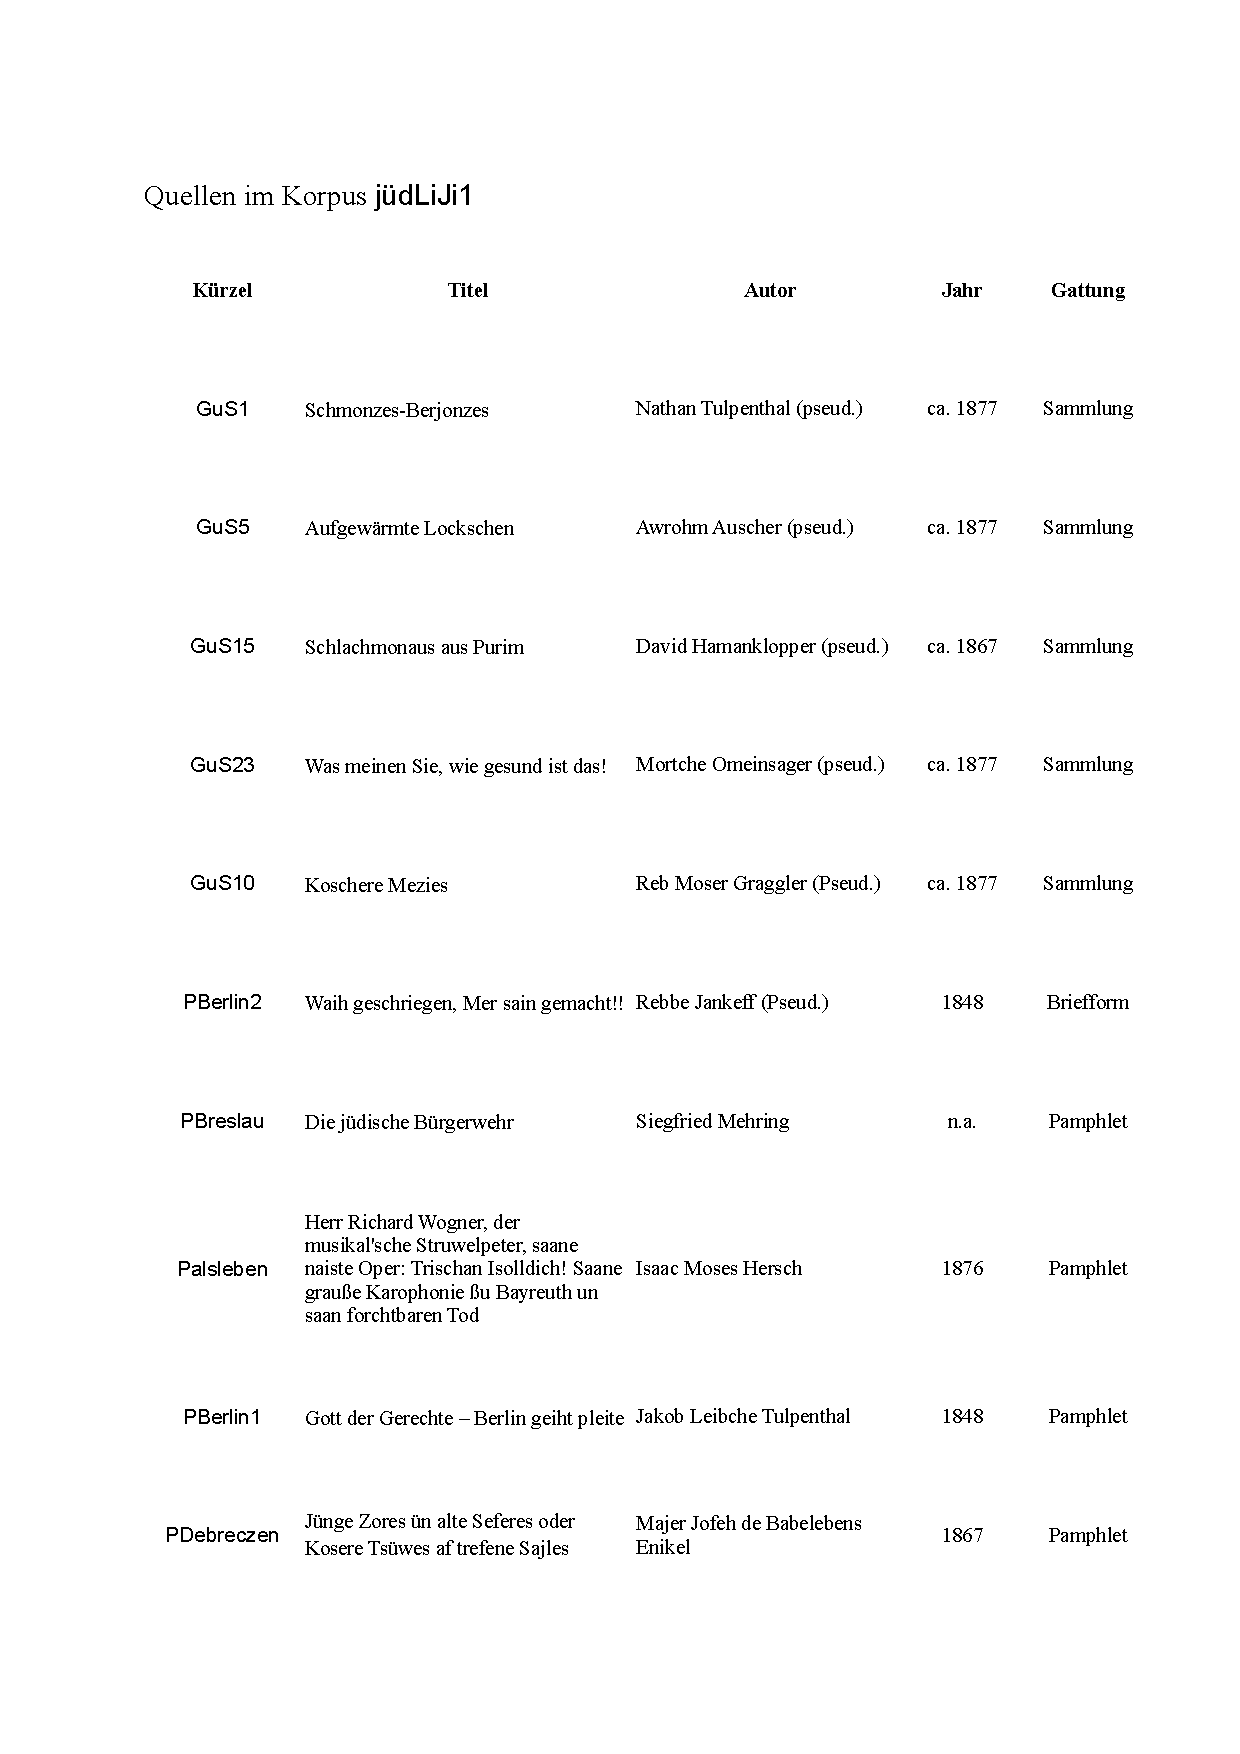
\includepdf[pages=-,pagecommand={\pagestyle{headings}}]{figures/Anhangju_liji1i.pdf} 
% % % % % 
%%%%%%%%%%%%%%%Quellen im \isi{Korpus} jüiJi1 ENDE
%%%%%%%%%%%%%%%%%%%%%%%%%%%%%%%%%%%%%%%%%%%%%
%%%%%%%%%%%%%%%%%%%%%%%%%%%%%%%%%%%%%%%%%%%%%
%%%%%%%%%%%%%%%%%%%%%%%%%%%%%%%%%%%%%%%%%%%%%%%%%%%%%%%%%%%%%%%%%%%%%%%%%%%%%%%
%%%%%%%%%%%%%%%%%%%%%%%%%%%%%%%%%%%%%%%%%%%%%%%%%%%%%%%%%%%%%%%%%%%%%%%%%%%%%%%
%%%Anfang  chr\ili{LiJi1} Phänomene     


%\section{Phänomentabelle \hai{chrLiJi1}} 
\newpage 
\phantomsection
\label{appendixphaenall}

\begin{footnotesize}\newgeometry{inner=9.4mm}
	\xhead{Phänomen & ab & ad & ah & aj & ak & ao & at & bp & bs & bw & dg & dk & dp & dw & ej & ev & fe & fl & fm & fs & gp & gw & hj & ia & jd & jk & jp & lb & lm & lp & lr & ls & ms & mv & nw & of & pa & pf & pg & pl & pm & pp & sb & sh & ss & sv & th & ut & vd & ve & wa & Σ}
	\xrow{V22 & - & \checkmark & - & \checkmark & \checkmark & \checkmark & \checkmark & \checkmark & - & \checkmark & - & \checkmark & \checkmark & \checkmark & \checkmark & - & \checkmark & \checkmark & - & - & \checkmark & - & \checkmark & \checkmark & - & \checkmark & \checkmark & \checkmark & \checkmark & - & \checkmark & \checkmark & \checkmark & \checkmark & \checkmark & \checkmark & \checkmark & \checkmark & \checkmark & - & \checkmark & - & - & \checkmark & \checkmark & \checkmark & \checkmark & - & \checkmark & - & \checkmark & 36} 
	\xrow{V12/13 & - & \checkmark & - & \checkmark & - & \checkmark & \checkmark & \checkmark & - & \checkmark & \checkmark & - & - & \checkmark & \checkmark & \checkmark & \checkmark & \checkmark & - & \checkmark & \checkmark & \checkmark & - & - & - & \checkmark & \checkmark & \checkmark & \checkmark & - & - & - & \checkmark & \checkmark & \checkmark & \checkmark & \checkmark & \checkmark & \checkmark & \checkmark & \checkmark & - & - & - & \checkmark & \checkmark & \checkmark & \checkmark & \checkmark & - & \checkmark & 34 } 
	\xrow{V24 & - & - & - & - & \checkmark & \checkmark & \checkmark & - & - & \checkmark & \checkmark & - & - & - & \checkmark & - & \checkmark & \checkmark & - & - & \checkmark & \checkmark & \checkmark & \checkmark & \checkmark & - & - & \checkmark & \checkmark & \checkmark & - & \checkmark & \checkmark & - & \checkmark & \checkmark & - & \checkmark & \checkmark & \checkmark & \checkmark & \checkmark & - & - & \checkmark & \checkmark & \checkmark & - & \checkmark & \checkmark & \checkmark & 31 } 
	\xrow{NP-Ex. & \checkmark & - & - & \checkmark & \checkmark & \checkmark & \checkmark & \checkmark & - & \checkmark & - & - & - & \checkmark & - & \checkmark & - & - & \checkmark & \checkmark & \checkmark & \checkmark & \checkmark & - & \checkmark & \checkmark & - & - & - & \checkmark & - & \checkmark & \checkmark & - & \checkmark & - & \checkmark & \checkmark & \checkmark & - & \checkmark & \checkmark & - & \checkmark & \checkmark & \checkmark & \checkmark & \checkmark & - & - & \checkmark & 31 } 
	\xrow{V44 & - & \checkmark & \checkmark & \checkmark & - & \checkmark & \checkmark & - & \checkmark & \checkmark & \checkmark & \checkmark & - & \checkmark & - & - & \checkmark & - & - & - & \checkmark & \checkmark & - & \checkmark & - & - & \checkmark & \checkmark & \checkmark & - & - & \checkmark & \checkmark & \checkmark & \checkmark & - & \checkmark & \checkmark & \checkmark & - & \checkmark & - & - & - & - & \checkmark & - & \checkmark & \checkmark & - & \checkmark & 29 } 
	\xrow{V42 & - & \checkmark & - & \checkmark & - & - & \checkmark & - & - & \checkmark & - & \checkmark & \checkmark & \checkmark & \checkmark & - & \checkmark & \checkmark & - & - & \checkmark & - & \checkmark & \checkmark & - & \checkmark & - & - & \checkmark & - & \checkmark & \checkmark & \checkmark & \checkmark & \checkmark & \checkmark & \checkmark & \checkmark & \checkmark & - & \checkmark & - & - & - & \checkmark & \checkmark & \checkmark & - & - & - & \checkmark & 29 } 
	\xrow{VR & \checkmark & \checkmark & - & \checkmark & \checkmark & \checkmark & \checkmark & \checkmark & - & \checkmark & - & - & - & - & - & \checkmark & \checkmark & - & - & \checkmark & - & - & \checkmark & - & \checkmark & \checkmark & \checkmark & - & - & \checkmark & \checkmark & \checkmark & - & - & \checkmark & - & \checkmark & \checkmark & \checkmark & - & \checkmark & \checkmark & - & \checkmark & \checkmark & \checkmark & \checkmark & - & - & - & \checkmark & 29 } 
	\xrow{PP-Ex. & \checkmark & - & - & \checkmark & \checkmark & \checkmark & \checkmark & \checkmark & - & \checkmark & - & - & - & - & - & - & \checkmark & - & \checkmark & \checkmark & \checkmark & \checkmark & \checkmark & - & \checkmark & \checkmark & - & - & - & \checkmark & - & \checkmark & \checkmark & - & \checkmark & - & \checkmark & \checkmark & \checkmark & - & \checkmark & \checkmark & - & \checkmark & - & \checkmark & \checkmark & \checkmark & - & - & \checkmark & 29 } 
	\xrow{V2 (dass) & \checkmark & \checkmark & - & \checkmark & \checkmark & \checkmark & \checkmark & \checkmark & - & \checkmark & - & - & - & \checkmark & - & \checkmark & \checkmark & - & - & \checkmark & - & - & \checkmark & - & \checkmark & \checkmark & \checkmark & - & - & \checkmark & - & \checkmark & - & - & \checkmark & \checkmark & \checkmark & \checkmark & - & - & - & \checkmark & - & \checkmark & \checkmark & \checkmark & - & \checkmark & - & - & \checkmark & 28 } 
	\xrow{V34 & - & \checkmark & - & \checkmark & \checkmark & \checkmark & - & - & - & - & \checkmark & \checkmark & \checkmark & - & \checkmark & \checkmark & \checkmark & - & - & - & - & \checkmark & - & - & - & \checkmark & \checkmark & - & - & - & - & \checkmark & \checkmark & \checkmark & - & - & \checkmark & - & - & - & - & - & \checkmark & - & \checkmark & \checkmark & \checkmark & \checkmark & \checkmark & - & - & 23 } 
	\xrow{\isi{Pluralsuffix} & \checkmark & \checkmark & - & \checkmark & - & - & - & - & - & \checkmark & - & - & - & \checkmark & - & - & - & \checkmark & - & - & - & - & \checkmark & - & \checkmark & \checkmark & \checkmark & - & \checkmark & - & - & - & - & \checkmark & \checkmark & - & \checkmark & - & \checkmark & - & - & \checkmark & - & - & - & \checkmark & \checkmark & - & \checkmark & - & - & 19 } 
	\xrow{AP-Ex. & - & - & - & \checkmark & \checkmark & \checkmark & \checkmark & - & - & \checkmark & - & - & - & - & - & \checkmark & - & - & - & \checkmark & - & - & - & - & \checkmark & \checkmark & - & - & - & \checkmark & - & \checkmark & - & - & \checkmark & - & \checkmark & - & - & - & - & - & - & \checkmark & - & \checkmark & \checkmark & \checkmark & - & - & \checkmark & 18 } 
	\xrow{o > u & - & \checkmark & \checkmark & - & \checkmark & \checkmark & - & - & - & - & - & - & - & \checkmark & - & - & \checkmark & \checkmark & - & \checkmark & - & \checkmark & - & \checkmark & - & \checkmark & - & - & - & - & - & - & \checkmark & \checkmark & - & - & \checkmark & - & - & - & - & - & - & - & \checkmark & \checkmark & - & - & \checkmark & - & - & 17 } 
	\xrow{Akk. n. Pr\"ap.& \checkmark & \checkmark & - & \checkmark & \checkmark & - & - & \checkmark & - & \checkmark & \checkmark & - & - & - & - & - & - & \checkmark & - & - & \checkmark & - & - & - & - & - & \checkmark & - & - & - & - & - & - & \checkmark & - & - & \checkmark & - & \checkmark & - & - & - & - & - & - & \checkmark & \checkmark & \checkmark & - & - & \checkmark & 17 } 
	\xrow{VPR & \checkmark & - & - & \checkmark & - & \checkmark & - & \checkmark & - & \checkmark & - & - & - & - & \checkmark & - & \checkmark & - & - & - & - & - & \checkmark & - & - & - & - & - & - & \checkmark & - & \checkmark & - & - & \checkmark & \checkmark & - & - & \checkmark & - & - & - & - & \checkmark & \checkmark & \checkmark & - & - & - & - & \checkmark & 17 } 
	\xrow{Zsf. V24,V44 & - & - & - & - & - & \checkmark & - & - & - & \checkmark & \checkmark & - & - & - & - & - & \checkmark & - & - & - & \checkmark & \checkmark & - & \checkmark & - & - & - & \checkmark & - & - & - & \checkmark & \checkmark & - & \checkmark & - & - & \checkmark & - & - & \checkmark & - & - & - & - & \checkmark & - & - & \checkmark & - & \checkmark & 16 } 
	\xrow{Pron. 1. Sg. Dat. & \checkmark & \checkmark & - & \checkmark & - & - & - & \checkmark & - & \checkmark & - & - & \checkmark & - & - & - & \checkmark & - & \checkmark & - & - & - & - & - & - & - & \checkmark & - & - & - & - & \checkmark & - & \checkmark & - & - & \checkmark & - & - & - & - & \checkmark & - & - & \checkmark & \checkmark & - & - & \checkmark & - & - & 16 } 
	\xrow{u > o & - & - & - & \checkmark & \checkmark & - & - & - & - & - & - & - & - & - & - & - & - & - & - & - & - & \checkmark & \checkmark & - & - & \checkmark & \checkmark & - & \checkmark & - & - & - & - & \checkmark & - & - & \checkmark & - & - & \checkmark & - & - & - & - & \checkmark & - & \checkmark & - & \checkmark & - & \checkmark & 14 } 
	\xrow{ue> i & - & \checkmark & - & - & \checkmark & - & \checkmark & - & - & - & \checkmark & - & - & - & - & - & - & - & - & - & - & \checkmark & - & - & - & - & \checkmark & - & - & - & - & - & \checkmark & \checkmark & - & - & \checkmark & - & - & - & - & \checkmark & - & - & \checkmark & \checkmark & \checkmark & - & \checkmark & - & - & 14 } 
	\xrow{Palat. & - & - & - & \checkmark & - & \checkmark & - & - & - & - & \checkmark & - & \checkmark & \checkmark & - & - & - & - & - & - & - & \checkmark & - & - & - & \checkmark & - & - & - & - & - & - & - & \checkmark & \checkmark & - & - & \checkmark & - & - & - & - & - & - & \checkmark & \checkmark & \checkmark & - & - & - & - & 13 } 
	\xrow{Akk. Pl. n.Pr\"ap. & - & \checkmark & - & \checkmark & \checkmark & - & - & \checkmark & - & - & \checkmark & - & - & - & - & - & - & \checkmark & - & - & \checkmark & - & - & - & - & - & - & - & - & - & - & - & \checkmark & - & - & - & - & - & \checkmark & - & - & - & - & - & - & - & \checkmark & \checkmark & \checkmark & - & \checkmark & 13 } 
	\xrow{scht (\isi{Auslaut}) & - & - & - & - & \checkmark & - & \checkmark & - & - & - & \checkmark & \checkmark & - & \checkmark & - & - & - & - & - & - & \checkmark & - & - & - & - & - & - & - & - & - & - & - & \checkmark & \checkmark & - & - & \checkmark & - & \checkmark & - & - & - & - & - & - & - & \checkmark & - & \checkmark & - & - & 12 } 
	\xrow{negative doubl. & - & - & - & - & \checkmark & - & - & - & - & \checkmark & \checkmark & - & \checkmark & - & - & - & \checkmark & - & - & - & \checkmark & - & - & - & - & - & - & - & - & - & - & - & - & \checkmark & \checkmark & - & \checkmark & - & \checkmark & - & - & - & \checkmark & - & - & \checkmark & - & - & - & - & - & 12 } 
	\xrow{VO \isi{Verbcluster} & - & - & - & - & - & \checkmark & \checkmark & - & - & - & - & - & - & - & - & - & - & - & - & - & - & - & - & - & - & \checkmark & \checkmark & - & - & - & - & \checkmark & \checkmark & - & - & - & - & - & \checkmark & - & - & \checkmark & - & - & - & \checkmark & \checkmark & - & \checkmark & - & - & 11 } 
	\xrow{ue > e & - & \checkmark & - & \checkmark & - & - & - & - & - & - & - & - & - & - & - & - & - & - & - & - & - & \checkmark & - & - & - & \checkmark & \checkmark & - & - & - & - & - & - & \checkmark & - & - & \checkmark & \checkmark & - & - & - & - & - & - & - & \checkmark & - & - & \checkmark & - & - & 10 } 
	\xrow{oe > e & - & - & - & - & \checkmark & - & - & - & - & - & - & - & - & - & - & - & \checkmark & - & \checkmark & - & - & \checkmark & - & - & - & - & \checkmark & - & - & - & - & - & - & - & - & - & \checkmark & - & - & - & - & - & - & - & \checkmark & \checkmark & \checkmark & - & \checkmark & - & - & 10 } 
	\xrow{Zsf. V22 & - & \checkmark & - & \checkmark & \checkmark & - & - & - & - & - & - & - & - & \checkmark & - & - & - & - & - & - & - & - & - & - & - & - & - & - & - & - & - & - & - & \checkmark & \checkmark & - & - & - & - & - & - & - & - & - & - & \checkmark & \checkmark & - & \checkmark & - & - & 9 } 
	\xrow{sein 'bin' & - & - & - & - & - & - & - & - & - & - & - & - & \checkmark & - & - & - & - & - & \checkmark & - & - & \checkmark & - & - & - & \checkmark & - & - & - & \checkmark & - & \checkmark & \checkmark & - & - & - & \checkmark & - & - & - & - & - & - & - & - & - & - & - & - & - & \checkmark & 9 } 
	\xrow{kommen Konstr. & - & - & - & \checkmark & - & \checkmark & - & - & - & - & \checkmark & - & - & - & - & - & - & - & - & - & \checkmark & - & - & - & - & - & - & - & - & \checkmark & - & - & - & \checkmark & - & - & - & - & \checkmark & - & - & \checkmark & - & - & - & - & - & - & \checkmark & - & - & 9 } 
	\xrow{Verbpartkl. & \checkmark & - & - & - & - & - & - & - & - & - & - & - & - & - & - & - & - & - & - & - & - & - & \checkmark & - & - & \checkmark & - & - & - & - & - & \checkmark & - & - & \checkmark & - & - & \checkmark & - & - & \checkmark & - & - & - & - & - & \checkmark & \checkmark & - & - & - & 9 } 
	\xrow{d statt t & - & \checkmark & - & - & - & - & - & - & - & - & - & - & - & \checkmark & - & - & - & - & - & - & - & - & - & - & - & - & - & - & - & - & - & - & - & - & - & \checkmark & - & - & \checkmark & \checkmark & - & - & - & - & - & - & \checkmark & \checkmark & \checkmark & - & - & 8 } 
	\xrow{k statt g & - & - & - & - & - & - & - & - & - & - & - & \checkmark & - & \checkmark & - & - & - & - & - & - & - & - & - & - & - & \checkmark & - & - & - & - & \checkmark & - & - & - & - & - & \checkmark & \checkmark & - & - & - & - & - & - & - & - & \checkmark & - & - & \checkmark & - & 8 } 
	\xrow{-lich Dim. Pl. & - & - & - & - & - & - & - & - & - & - & \checkmark & - & - & - & - & - & - & - & - & - & \checkmark & \checkmark & - & - & - & - & - & - & \checkmark & - & - & - & - & - & - & - & \checkmark & - & \checkmark & - & - & - & - & - & - & \checkmark & - & - & - & - & - & 7 } 
	\xrow{Pron. 2. Sg. Dat. & - & \checkmark & - & \checkmark & - & - & - & - & - & \checkmark & - & - & - & - & - & - & - & - & - & - & - & - & - & - & - & - & \checkmark & - & - & - & - & - & - & - & - & - & \checkmark & - & - & - & - & - & - & - & - & - & - & \checkmark & \checkmark & - & - & 7 } 
	\xrow{Rel.-partkl. wo & - & - & - & - & - & - & - & - & - & - & - & - & - & - & - & - & \checkmark & - & - & - & - & \checkmark & - & - & - & - & - & - & \checkmark & - & - & \checkmark & - & - & - & - & \checkmark & - & \checkmark & - & - & - & - & - & - & \checkmark & - & - & - & - & - & 7 } 
	\xrow{Pron. H\"ofl. Akk. & - & \checkmark & - & - & - & - & - & \checkmark & - & - & - & - & - & - & - & - & - & - & - & - & - & \checkmark & - & - & - & - & \checkmark & - & - & \checkmark & - & - & - & - & - & - & \checkmark & - & - & - & - & - & - & - & - & - & - & - & - & - & - & 6 } 
	\xrow{V2 (weil) & - & - & - & - & - & - & - & - & - & - & - & - & - & - & - & - & - & - & - & - & - & - & - & - & \checkmark & - & - & - & - & \checkmark & - & \checkmark & - & - & - & - & - & \checkmark & - & - & - & - & - & \checkmark & - & - & \checkmark & - & - & - & - & 6 } 
	\xrow{Adv.-Ex. & - & - & - & - & - & - & - & - & - & \checkmark & - & - & - & - & - & - & - & - & \checkmark & - & - & - & \checkmark & - & - & - & - & - & - & - & - & - & - & - & - & - & - & - & - & - & - & \checkmark & - & \checkmark & - & - & \checkmark & - & - & - & - & 6 } 
	\xrow{s statt z & - & - & - & - & - & - & - & - & - & \checkmark & - & - & - & - & - & - & - & - & - & - & - & - & - & - & - & - & - & - & - & - & - & - & - & - & - & - & \checkmark & \checkmark & - & - & - & - & - & - & - & - & \checkmark & - & \checkmark & - & - & 5 } 
	\xrow{ge- \isi{Partizip} & - & - & - & \checkmark & - & - & - & - & - & - & - & - & - & - & - & - & \checkmark & \checkmark & - & - & - & - & - & - & - & - & - & - & \checkmark & - & - & - & - & \checkmark & - & - & - & - & - & - & - & - & - & - & - & - & - & - & - & - & - & 5 } 
	\xrow{Dat. n. Pr\"ap & - & - & - & - & - & - & - & - & - & - & - & - & - & - & - & - & - & - & - & - & - & \checkmark & - & - & - & - & - & - & \checkmark & - & - & - & - & - & - & - & - & - & \checkmark & - & - & - & - & - & \checkmark & - & - & - & \checkmark & - & - & 5 } 
	\xrow{Pron. 1. Pl. Nom. & - & - & - & - & \checkmark & - & - & - & - & - & - & - & - & - & - & - & - & \checkmark & - & - & - & \checkmark & - & - & - & - & \checkmark & - & - & - & - & - & - & - & - & - & - & - & - & - & - & - & - & - & - & \checkmark & - & - & - & - & - & 5 } 
	\xrow{Pron. H\"ofl. Nom. & \checkmark & - & - & - & - & \checkmark & - & - & - & - & - & - & - & - & - & - & \checkmark & - & \checkmark & - & - & - & - & - & - & \checkmark & - & - & - & - & - & - & - & - & - & - & - & - & - & - & - & - & - & - & - & - & - & - & - & - & - & 5 } 
	\xrow{p statt b & - & - & - & \checkmark & - & - & - & - & \checkmark & - & - & - & - & - & - & - & - & - & - & - & - & \checkmark & - & - & - & - & \checkmark & - & - & - & - & - & - & - & - & - & - & - & - & - & - & - & - & - & - & - & - & - & - & - & - & 4 } 
	\xrow{no-IPP & - & - & - & - & \checkmark & - & - & - & - & - & - & - & - & - & - & - & \checkmark & - & - & - & - & - & - & - & - & - & - & - & - & - & - & - & - & \checkmark & - & - & - & \checkmark & - & - & - & - & - & - & - & - & - & - & - & - & - & 4 } 
	\xrow{b statt p & - & - & - & - & - & - & - & - & - & - & - & - & - & - & - & - & - & - & - & - & - & - & - & - & - & - & - & - & - & - & - & - & - & - & - & \checkmark & - & - & \checkmark & - & - & - & - & - & - & - & - & - & \checkmark & - & - & 3 } 
	\xrow{germ. *-pp- & - & - & - & - & - & - & - & - & - & - & - & - & - & - & - & - & - & \checkmark & - & - & - & - & - & - & - & - & - & - & - & - & - & - & - & \checkmark & - & - & - & - & - & - & - & - & - & - & - & \checkmark & - & - & - & - & - & 3 } 
	\xrow{oj. \isi{Genus} & - & - & - & - & - & - & - & - & \checkmark & - & - & - & - & - & - & - & - & - & - & - & - & - & - & - & - & - & - & - & - & - & \checkmark & - & - & - & - & - & - & - & - & - & - & - & - & - & \checkmark & - & - & - & - & - & - & 3 } 
	\xrow{Nom. Sg. m. NP & - & - & - & - & \checkmark & - & - & - & - & - & - & - & - & - & - & - & - & - & - & \checkmark & - & - & - & - & - & - & - & - & - & - & - & \checkmark & - & - & - & - & - & - & - & - & - & - & - & - & - & - & - & - & - & - & - & 3 } 
	\xrow{Pron. 1. Sg. Akk. & - & - & - & - & - & \checkmark & - & - & - & - & - & - & - & - & - & - & - & - & - & - & - & - & - & - & - & - & - & - & - & - & - & - & - & - & - & - & - & - & - & - & - & - & - & - & - & - & \checkmark & \checkmark & - & - & - & 3 } 
	\xrow{Rel.-partkl. was & - & - & - & - & - & - & - & \checkmark & - & - & - & - & - & - & - & - & - & - & - & - & - & \checkmark & - & - & - & - & - & - & - & - & - & - & - & - & - & - & - & - & - & - & - & - & - & - & - & \checkmark & - & - & - & - & - & 3 } 
	\xrow{w statt b & - & - & - & - & - & - & - & - & - & - & - & - & - & - & - & - & - & - & - & - & - & - & - & - & - & - & - & - & - & - & - & - & - & - & - & - & - & - & - & - & - & - & - & - & - & \checkmark & - & - & \checkmark & - & - & 2 } 
	\xrow{Dat. Pl. n. Pr\"ap.& - & - & - & - & - & - & - & - & - & - & - & - & - & - & - & - & - & - & - & - & - & - & - & - & - & - & - & - & - & - & - & - & - & - & - & - & - & - & - & - & - & \checkmark & - & - & - & - & - & - & - & - & \checkmark & 2 } 
	\xrow{oe > i & - & - & - & - & - & - & - & - & - & - & - & - & - & - & - & - & - & - & - & - & - & - & - & - & - & - & - & - & - & - & - & - & - & - & - & - & - & - & \checkmark & - & - & - & - & - & - & - & - & - & - & - & - & 1 } 
	\xrow{scht (\isi{Anlaut}) & - & - & - & - & - & - & - & - & - & - & - & - & - & - & - & - & - & - & - & - & - & - & - & - & - & - & - & - & - & - & - & - & - & - & - & - & - & - & - & - & - & - & - & - & - & - & - & \checkmark & - & - & - & 1 } 
	\xrow{Dat. Sg. m. NP & - & - & - & - & - & - & - & - & - & - & - & - & - & - & - & - & - & - & - & - & - & - & - & - & - & - & - & - & - & - & - & - & - & - & - & - & - & - & - & - & - & - & - & - & \checkmark & - & - & - & - & - & - & 1 } 
	\xrow{Nom. Pl. NP & - & - & - & - & - & - & - & - & - & - & - & - & - & - & - & - & - & - & - & - & - & - & - & - & - & - & - & - & - & - & - & \checkmark & - & - & - & - & - & - & - & - & - & - & - & - & - & - & - & - & - & - & - & 1 } 
	\xrow{Pron. 3. Sg. Akk. & - & - & - & - & - & - & - & - & - & - & - & - & - & - & - & - & - & - & - & - & - & - & - & - & - & - & - & - & - & - & - & - & - & - & - & - & - & - & - & - & - & - & - & - & - & \checkmark & - & - & - & - & - & 1 }
	\xfinish
\end{footnotesize}\restoregeometry

%\begin{table}\footnotesize
%%\caption*{Phänomene im \hai{chrLiJi1} %!!!!!!!! CAPTION & LABEL AUS PDF ÜBERNEHMEN   !!!!!!!!!!
%\begin{tabular}{  l  l  l  l  l  l  l  l  l  l  l  l  l  l  l  l  l  l  l  l  l  l  l  l  l  l  l  l  l  l  l  l  l  l  l  l  l  l  l  l  l  l  l  l  l  l  l  l  l  l  l  l  l  }
%\lsptoprule
%	                                           Phänomen         & AB & AD & AH & AJ & AK & AO & AT & BP & BS & BW & DG & DK & DP & DW & EJ & EV & FE & FL & FM & FS & GP & GW & HJ & IA & JD & JK & JP & LB & LM & LP & LR & LS & MS & MV & NW & OF & PA & PF & PG & PL & PM & PP & SB & SH & SS & SV & TH & UT & VD & VE & WA & SUMME \\  \midrule
%	V22 & - & \checkmark & - & \checkmark & \checkmark & \checkmark & \checkmark & \checkmark & - & \checkmark & - & \checkmark & \checkmark & \checkmark & \checkmark & - & \checkmark & \checkmark & - & - & \checkmark & - & \checkmark & \checkmark & - & \checkmark & \checkmark & \checkmark & \checkmark & - & \checkmark & \checkmark & \checkmark & \checkmark & \checkmark & \checkmark & \checkmark & \checkmark & \checkmark & - & \checkmark & - & - & \checkmark & \checkmark & \checkmark & \checkmark & - & \checkmark & - & \checkmark & 36 \\ 
%	V12\checkmark13 & - & \checkmark & - & \checkmark & - & \checkmark & \checkmark & \checkmark & - & \checkmark & \checkmark & - & - & \checkmark & \checkmark & \checkmark & \checkmark & \checkmark & - & \checkmark & \checkmark & \checkmark & - & - & - & \checkmark & \checkmark & \checkmark & \checkmark & - & - & - & \checkmark & \checkmark & \checkmark & \checkmark & \checkmark & \checkmark & \checkmark & \checkmark & \checkmark & - & - & - & \checkmark & \checkmark & \checkmark & \checkmark & \checkmark & - & \checkmark & 34 \\ 
%	V24 & - & - & - & - & \checkmark & \checkmark & \checkmark & - & - & \checkmark & \checkmark & - & - & - & \checkmark & - & \checkmark & \checkmark & - & - & \checkmark & \checkmark & \checkmark & \checkmark & \checkmark & - & - & \checkmark & \checkmark & \checkmark & - & \checkmark & \checkmark & - & \checkmark & \checkmark & - & \checkmark & \checkmark & \checkmark & \checkmark & \checkmark & - & - & \checkmark & \checkmark & \checkmark & - & \checkmark & \checkmark & \checkmark & 31 \\ 
%	NP-Ex. & \checkmark & - & - & \checkmark & \checkmark & \checkmark & \checkmark & \checkmark & - & \checkmark & - & - & - & \checkmark & - & \checkmark & - & - & \checkmark & \checkmark & \checkmark & \checkmark & \checkmark & - & \checkmark & \checkmark & - & - & - & \checkmark & - & \checkmark & \checkmark & - & \checkmark & - & \checkmark & \checkmark & \checkmark & - & \checkmark & \checkmark & - & \checkmark & \checkmark & \checkmark & \checkmark & \checkmark & - & - & \checkmark & 31 \\ 
%	V44 & - & \checkmark & \checkmark & \checkmark & - & \checkmark & \checkmark & - & \checkmark & \checkmark & \checkmark & \checkmark & - & \checkmark & - & - & \checkmark & - & - & - & \checkmark & \checkmark & - & \checkmark & - & - & \checkmark & \checkmark & \checkmark & - & - & \checkmark & \checkmark & \checkmark & \checkmark & - & \checkmark & \checkmark & \checkmark & - & \checkmark & - & - & - & - & \checkmark & - & \checkmark & \checkmark & - & \checkmark & 29 \\ 
%	V42 & - & \checkmark & - & \checkmark & - & - & \checkmark & - & - & \checkmark & - & \checkmark & \checkmark & \checkmark & \checkmark & - & \checkmark & \checkmark & - & - & \checkmark & - & \checkmark & \checkmark & - & \checkmark & - & - & \checkmark & - & \checkmark & \checkmark & \checkmark & \checkmark & \checkmark & \checkmark & \checkmark & \checkmark & \checkmark & - & \checkmark & - & - & - & \checkmark & \checkmark & \checkmark & - & - & - & \checkmark & 29 \\ 
%	VR & \checkmark & \checkmark & - & \checkmark & \checkmark & \checkmark & \checkmark & \checkmark & - & \checkmark & - & - & - & - & - & \checkmark & \checkmark & - & - & \checkmark & - & - & \checkmark & - & \checkmark & \checkmark & \checkmark & - & - & \checkmark & \checkmark & \checkmark & - & - & \checkmark & - & \checkmark & \checkmark & \checkmark & - & \checkmark & \checkmark & - & \checkmark & \checkmark & \checkmark & \checkmark & - & - & - & \checkmark & 29 \\ 
%	PP-Ex. & \checkmark & - & - & \checkmark & \checkmark & \checkmark & \checkmark & \checkmark & - & \checkmark & - & - & - & - & - & - & \checkmark & - & \checkmark & \checkmark & \checkmark & \checkmark & \checkmark & - & \checkmark & \checkmark & - & - & - & \checkmark & - & \checkmark & \checkmark & - & \checkmark & - & \checkmark & \checkmark & \checkmark & - & \checkmark & \checkmark & - & \checkmark & - & \checkmark & \checkmark & \checkmark & - & - & \checkmark & 29 \\ 
%	V2 (dass) & \checkmark & \checkmark & - & \checkmark & \checkmark & \checkmark & \checkmark & \checkmark & - & \checkmark & - & - & - & \checkmark & - & \checkmark & \checkmark & - & - & \checkmark & - & - & \checkmark & - & \checkmark & \checkmark & \checkmark & - & - & \checkmark & - & \checkmark & - & - & \checkmark & \checkmark & \checkmark & \checkmark & - & - & - & \checkmark & - & \checkmark & \checkmark & \checkmark & - & \checkmark & - & - & \checkmark & 28 \\ 
%	V34 & - & \checkmark & - & \checkmark & \checkmark & \checkmark & - & - & - & - & \checkmark & \checkmark & \checkmark & - & \checkmark & \checkmark & \checkmark & - & - & - & - & \checkmark & - & - & - & \checkmark & \checkmark & - & - & - & - & \checkmark & \checkmark & \checkmark & - & - & \checkmark & - & - & - & - & - & \checkmark & - & \checkmark & \checkmark & \checkmark & \checkmark & \checkmark & - & - & 23 \\ 
%	\isi{Pluralsuffix} & \checkmark & \checkmark & - & \checkmark & - & - & - & - & - & \checkmark & - & - & - & \checkmark & - & - & - & \checkmark & - & - & - & - & \checkmark & - & \checkmark & \checkmark & \checkmark & - & \checkmark & - & - & - & - & \checkmark & \checkmark & - & \checkmark & - & \checkmark & - & - & \checkmark & - & - & - & \checkmark & \checkmark & - & \checkmark & - & - & 19 \\ 
%	AP-Ex. & - & - & - & \checkmark & \checkmark & \checkmark & \checkmark & - & - & \checkmark & - & - & - & - & - & \checkmark & - & - & - & \checkmark & - & - & - & - & \checkmark & \checkmark & - & - & - & \checkmark & - & \checkmark & - & - & \checkmark & - & \checkmark & - & - & - & - & - & - & \checkmark & - & \checkmark & \checkmark & \checkmark & - & - & \checkmark & 18 \\ 
%	o > u & - & \checkmark & \checkmark & - & \checkmark & \checkmark & - & - & - & - & - & - & - & \checkmark & - & - & \checkmark & \checkmark & - & \checkmark & - & \checkmark & - & \checkmark & - & \checkmark & - & - & - & - & - & - & \checkmark & \checkmark & - & - & \checkmark & - & - & - & - & - & - & - & \checkmark & \checkmark & - & - & \checkmark & - & - & 17 \\ 
%	Kasus n. PrŠp. Akk. statt Dat. & \checkmark & \checkmark & - & \checkmark & \checkmark & - & - & \checkmark & - & \checkmark & \checkmark & - & - & - & - & - & - & \checkmark & - & - & \checkmark & - & - & - & - & - & \checkmark & - & - & - & - & - & - & \checkmark & - & - & \checkmark & - & \checkmark & - & - & - & - & - & - & \checkmark & \checkmark & \checkmark & - & - & \checkmark & 17 \\ 
%	VPR & \checkmark & - & - & \checkmark & - & \checkmark & - & \checkmark & - & \checkmark & - & - & - & - & \checkmark & - & \checkmark & - & - & - & - & - & \checkmark & - & - & - & - & - & - & \checkmark & - & \checkmark & - & - & \checkmark & \checkmark & - & - & \checkmark & - & - & - & - & \checkmark & \checkmark & \checkmark & - & - & - & - & \checkmark & 17 \\ 
%	\isi{Zusammenfall} V24,V44 & - & - & - & - & - & \checkmark & - & - & - & \checkmark & \checkmark & - & - & - & - & - & \checkmark & - & - & - & \checkmark & \checkmark & - & \checkmark & - & - & - & \checkmark & - & - & - & \checkmark & \checkmark & - & \checkmark & - & - & \checkmark & - & - & \checkmark & - & - & - & - & \checkmark & - & - & \checkmark & - & \checkmark & 16 \\ 
%	Pronomen1. Sg. Dat. & \checkmark & \checkmark & - & \checkmark & - & - & - & \checkmark & - & \checkmark & - & - & \checkmark & - & - & - & \checkmark & - & \checkmark & - & - & - & - & - & - & - & \checkmark & - & - & - & - & \checkmark & - & \checkmark & - & - & \checkmark & - & - & - & - & \checkmark & - & - & \checkmark & \checkmark & - & - & \checkmark & - & - & 16 \\ 
%	u > o & - & - & - & \checkmark & \checkmark & - & - & - & - & - & - & - & - & - & - & - & - & - & - & - & - & \checkmark & \checkmark & - & - & \checkmark & \checkmark & - & \checkmark & - & - & - & - & \checkmark & - & - & \checkmark & - & - & \checkmark & - & - & - & - & \checkmark & - & \checkmark & - & \checkmark & - & \checkmark & 14 \\ 
%	ue> i & - & \checkmark & - & - & \checkmark & - & \checkmark & - & - & - & \checkmark & - & - & - & - & - & - & - & - & - & - & \checkmark & - & - & - & - & \checkmark & - & - & - & - & - & \checkmark & \checkmark & - & - & \checkmark & - & - & - & - & \checkmark & - & - & \checkmark & \checkmark & \checkmark & - & \checkmark & - & - & 14 \\ 
%	\isi{Palatalisierung} & - & - & - & \checkmark & - & \checkmark & - & - & - & - & \checkmark & - & \checkmark & \checkmark & - & - & - & - & - & - & - & \checkmark & - & - & - & \checkmark & - & - & - & - & - & - & - & \checkmark & \checkmark & - & - & \checkmark & - & - & - & - & - & - & \checkmark & \checkmark & \checkmark & - & - & - & - & 13 \\ 
%	Kasus n. PrŠp. Pl. Akk. Statt Dat. & - & \checkmark & - & \checkmark & \checkmark & - & - & \checkmark & - & - & \checkmark & - & - & - & - & - & - & \checkmark & - & - & \checkmark & - & - & - & - & - & - & - & - & - & - & - & \checkmark & - & - & - & - & - & \checkmark & - & - & - & - & - & - & - & \checkmark & \checkmark & \checkmark & - & \checkmark & 13 \\ 
%	scht (\isi{Auslaut}) & - & - & - & - & \checkmark & - & \checkmark & - & - & - & \checkmark & \checkmark & - & \checkmark & - & - & - & - & - & - & \checkmark & - & - & - & - & - & - & - & - & - & - & - & \checkmark & \checkmark & - & - & \checkmark & - & \checkmark & - & - & - & - & - & - & - & \checkmark & - & \checkmark & - & - & 12 \\ 
%	\isi{negative doubling} & - & - & - & - & \checkmark & - & - & - & - & \checkmark & \checkmark & - & \checkmark & - & - & - & \checkmark & - & - & - & \checkmark & - & - & - & - & - & - & - & - & - & - & - & - & \checkmark & \checkmark & - & \checkmark & - & \checkmark & - & - & - & \checkmark & - & - & \checkmark & - & - & - & - & - & 12 \\ 
%	1-2-3 \isi{Verbcluster} & - & - & - & - & - & \checkmark & \checkmark & - & - & - & - & - & - & - & - & - & - & - & - & - & - & - & - & - & - & \checkmark & \checkmark & - & - & - & - & \checkmark & \checkmark & - & - & - & - & - & \checkmark & - & - & \checkmark & - & - & - & \checkmark & \checkmark & - & \checkmark & - & - & 11 \\ 
%	ue > e & - & \checkmark & - & \checkmark & - & - & - & - & - & - & - & - & - & - & - & - & - & - & - & - & - & \checkmark & - & - & - & \checkmark & \checkmark & - & - & - & - & - & - & \checkmark & - & - & \checkmark & \checkmark & - & - & - & - & - & - & - & \checkmark & - & - & \checkmark & - & - & 10 \\ 
%	oe > e & - & - & - & - & \checkmark & - & - & - & - & - & - & - & - & - & - & - & \checkmark & - & \checkmark & - & - & \checkmark & - & - & - & - & \checkmark & - & - & - & - & - & - & - & - & - & \checkmark & - & - & - & - & - & - & - & \checkmark & \checkmark & \checkmark & - & \checkmark & - & - & 10 \\ 
%	\isi{Zusammenfall} V22 & - & \checkmark & - & \checkmark & \checkmark & - & - & - & - & - & - & - & - & \checkmark & - & - & - & - & - & - & - & - & - & - & - & - & - & - & - & - & - & - & - & \checkmark & \checkmark & - & - & - & - & - & - & - & - & - & - & \checkmark & \checkmark & - & \checkmark & - & - & 9 \\ 
%	sein 'bin' & - & - & - & - & - & - & - & - & - & - & - & - & \checkmark & - & - & - & - & - & \checkmark & - & - & \checkmark & - & - & - & \checkmark & - & - & - & \checkmark & - & \checkmark & \checkmark & - & - & - & \checkmark & - & - & - & - & - & - & - & - & - & - & - & - & - & \checkmark & 9 \\ 
%	kommen-zu-gehen & - & - & - & \checkmark & - & \checkmark & - & - & - & - & \checkmark & - & - & - & - & - & - & - & - & - & \checkmark & - & - & - & - & - & - & - & - & \checkmark & - & - & - & \checkmark & - & - & - & - & \checkmark & - & - & \checkmark & - & - & - & - & - & - & \checkmark & - & - & 9 \\ 
%	\isi{Verbpartikel} rechtsadjazent & \checkmark & - & - & - & - & - & - & - & - & - & - & - & - & - & - & - & - & - & - & - & - & - & \checkmark & - & - & \checkmark & - & - & - & - & - & \checkmark & - & - & \checkmark & - & - & \checkmark & - & - & \checkmark & - & - & - & - & - & \checkmark & \checkmark & - & - & - & 9 \\ 
%	d statt t & - & \checkmark & - & - & - & - & - & - & - & - & - & - & - & \checkmark & - & - & - & - & - & - & - & - & - & - & - & - & - & - & - & - & - & - & - & - & - & \checkmark & - & - & \checkmark & \checkmark & - & - & - & - & - & - & \checkmark & \checkmark & \checkmark & - & - & 8 \\ 
%	k statt g & - & - & - & - & - & - & - & - & - & - & - & \checkmark & - & \checkmark & - & - & - & - & - & - & - & - & - & - & - & \checkmark & - & - & - & - & \checkmark & - & - & - & - & - & \checkmark & \checkmark & - & - & - & - & - & - & - & - & \checkmark & - & - & \checkmark & - & 8 \\ 
%	lich Dim. Pl. & - & - & - & - & - & - & - & - & - & - & \checkmark & - & - & - & - & - & - & - & - & - & \checkmark & \checkmark & - & - & - & - & - & - & \checkmark & - & - & - & - & - & - & - & \checkmark & - & \checkmark & - & - & - & - & - & - & \checkmark & - & - & - & - & - & 7 \\ 
%	\isi{Pronomen} 2. Sg. Dat. & - & \checkmark & - & \checkmark & - & - & - & - & - & \checkmark & - & - & - & - & - & - & - & - & - & - & - & - & - & - & - & - & \checkmark & - & - & - & - & - & - & - & - & - & \checkmark & - & - & - & - & - & - & - & - & - & - & \checkmark & \checkmark & - & - & 7 \\ 
%	\isi{Relativpartikel} wo & - & - & - & - & - & - & - & - & - & - & - & - & - & - & - & - & \checkmark & - & - & - & - & \checkmark & - & - & - & - & - & - & \checkmark & - & - & \checkmark & - & - & - & - & \checkmark & - & \checkmark & - & - & - & - & - & - & \checkmark & - & - & - & - & - & 7 \\ 
%	\isi{Pronomen} Hšfl. Akk. & - & \checkmark & - & - & - & - & - & \checkmark & - & - & - & - & - & - & - & - & - & - & - & - & - & \checkmark & - & - & - & - & \checkmark & - & - & \checkmark & - & - & - & - & - & - & \checkmark & - & - & - & - & - & - & - & - & - & - & - & - & - & - & 6 \\ 
%	V2 (weil) & - & - & - & - & - & - & - & - & - & - & - & - & - & - & - & - & - & - & - & - & - & - & - & - & \checkmark & - & - & - & - & \checkmark & - & \checkmark & - & - & - & - & - & \checkmark & - & - & - & - & - & \checkmark & - & - & \checkmark & - & - & - & - & 6 \\ 
%	ADV-Ex. & - & - & - & - & - & - & - & - & - & \checkmark & - & - & - & - & - & - & - & - & \checkmark & - & - & - & \checkmark & - & - & - & - & - & - & - & - & - & - & - & - & - & - & - & - & - & - & \checkmark & - & \checkmark & - & - & \checkmark & - & - & - & - & 6 \\ 
%	s statt z & - & - & - & - & - & - & - & - & - & \checkmark & - & - & - & - & - & - & - & - & - & - & - & - & - & - & - & - & - & - & - & - & - & - & - & - & - & - & \checkmark & \checkmark & - & - & - & - & - & - & - & - & \checkmark & - & \checkmark & - & - & 5 \\ 
%	ge- \isi{Partizip} & - & - & - & \checkmark & - & - & - & - & - & - & - & - & - & - & - & - & \checkmark & \checkmark & - & - & - & - & - & - & - & - & - & - & \checkmark & - & - & - & - & \checkmark & - & - & - & - & - & - & - & - & - & - & - & - & - & - & - & - & - & 5 \\ 
%	Kasus n. PrŠp- Dat. statt Akk. & - & - & - & - & - & - & - & - & - & - & - & - & - & - & - & - & - & - & - & - & - & \checkmark & - & - & - & - & - & - & \checkmark & - & - & - & - & - & - & - & - & - & \checkmark & - & - & - & - & - & \checkmark & - & - & - & \checkmark & - & - & 5 \\ 
%	\isi{Pronomen} 1. Pl. Nom. = 1. Sg. Dat. & - & - & - & - & \checkmark & - & - & - & - & - & - & - & - & - & - & - & - & \checkmark & - & - & - & \checkmark & - & - & - & - & \checkmark & - & - & - & - & - & - & - & - & - & - & - & - & - & - & - & - & - & - & \checkmark & - & - & - & - & - & 5 \\ 
%	\isi{Pronomen} Hšfl. Nom. & \checkmark & - & - & - & - & \checkmark & - & - & - & - & - & - & - & - & - & - & \checkmark & - & \checkmark & - & - & - & - & - & - & \checkmark & - & - & - & - & - & - & - & - & - & - & - & - & - & - & - & - & - & - & - & - & - & - & - & - & - & 5 \\ 
%	p statt b & - & - & - & \checkmark & - & - & - & - & \checkmark & - & - & - & - & - & - & - & - & - & - & - & - & \checkmark & - & - & - & - & \checkmark & - & - & - & - & - & - & - & - & - & - & - & - & - & - & - & - & - & - & - & - & - & - & - & - & 4 \\ 
%	no-IPP & - & - & - & - & \checkmark & - & - & - & - & - & - & - & - & - & - & - & \checkmark & - & - & - & - & - & - & - & - & - & - & - & - & - & - & - & - & \checkmark & - & - & - & \checkmark & - & - & - & - & - & - & - & - & - & - & - & - & - & 4 \\ 
%	b statt p & - & - & - & - & - & - & - & - & - & - & - & - & - & - & - & - & - & - & - & - & - & - & - & - & - & - & - & - & - & - & - & - & - & - & - & \checkmark & - & - & \checkmark & - & - & - & - & - & - & - & - & - & \checkmark & - & - & 3 \\ 
%	germ. *-pp- & - & - & - & - & - & - & - & - & - & - & - & - & - & - & - & - & - & \checkmark & - & - & - & - & - & - & - & - & - & - & - & - & - & - & - & \checkmark & - & - & - & - & - & - & - & - & - & - & - & \checkmark & - & - & - & - & - & 3 \\ 
%	oj. \isi{Genus} & - & - & - & - & - & - & - & - & \checkmark & - & - & - & - & - & - & - & - & - & - & - & - & - & - & - & - & - & - & - & - & - & \checkmark & - & - & - & - & - & - & - & - & - & - & - & - & - & \checkmark & - & - & - & - & - & - & 3 \\ 
%	Kasus volle NP Sg. m. Nom. & - & - & - & - & \checkmark & - & - & - & - & - & - & - & - & - & - & - & - & - & - & \checkmark & - & - & - & - & - & - & - & - & - & - & - & \checkmark & - & - & - & - & - & - & - & - & - & - & - & - & - & - & - & - & - & - & - & 3 \\ 
%	\isi{Pronomen} 1. Sg. Akk. & - & - & - & - & - & \checkmark & - & - & - & - & - & - & - & - & - & - & - & - & - & - & - & - & - & - & - & - & - & - & - & - & - & - & - & - & - & - & - & - & - & - & - & - & - & - & - & - & \checkmark & \checkmark & - & - & - & 3 \\ 
%	\isi{Relativpartikel} was & - & - & - & - & - & - & - & \checkmark & - & - & - & - & - & - & - & - & - & - & - & - & - & \checkmark & - & - & - & - & - & - & - & - & - & - & - & - & - & - & - & - & - & - & - & - & - & - & - & \checkmark & - & - & - & - & - & 3 \\ 
%	w statt b & - & - & - & - & - & - & - & - & - & - & - & - & - & - & - & - & - & - & - & - & - & - & - & - & - & - & - & - & - & - & - & - & - & - & - & - & - & - & - & - & - & - & - & - & - & \checkmark & - & - & \checkmark & - & - & 2 \\ 
%	Kasus n. PrŠp. Pl. Dat. & - & - & - & - & - & - & - & - & - & - & - & - & - & - & - & - & - & - & - & - & - & - & - & - & - & - & - & - & - & - & - & - & - & - & - & - & - & - & - & - & - & \checkmark & - & - & - & - & - & - & - & - & \checkmark & 2 \\ 
%	oe > i & - & - & - & - & - & - & - & - & - & - & - & - & - & - & - & - & - & - & - & - & - & - & - & - & - & - & - & - & - & - & - & - & - & - & - & - & - & - & \checkmark & - & - & - & - & - & - & - & - & - & - & - & - & 1 \\ 
%	scht (\isi{Anlaut}) & - & - & - & - & - & - & - & - & - & - & - & - & - & - & - & - & - & - & - & - & - & - & - & - & - & - & - & - & - & - & - & - & - & - & - & - & - & - & - & - & - & - & - & - & - & - & - & \checkmark & - & - & - & 1 \\ 
%	Kasus volle NP Sg. M. Dat. & - & - & - & - & - & - & - & - & - & - & - & - & - & - & - & - & - & - & - & - & - & - & - & - & - & - & - & - & - & - & - & - & - & - & - & - & - & - & - & - & - & - & - & - & \checkmark & - & - & - & - & - & - & 1 \\ 
%	Kasus volle NP Pl. Nom. & - & - & - & - & - & - & - & - & - & - & - & - & - & - & - & - & - & - & - & - & - & - & - & - & - & - & - & - & - & - & - & \checkmark & - & - & - & - & - & - & - & - & - & - & - & - & - & - & - & - & - & - & - & 1 \\ 
%	\isi{Pronomen} 3. Sg. Akk. & - & - & - & - & - & - & - & - & - & - & - & - & - & - & - & - & - & - & - & - & - & - & - & - & - & - & - & - & - & - & - & - & - & - & - & - & - & - & - & - & - & - & - & - & - & \checkmark & - & - & - & - & - & 1 \\ 
%
%
%\lspbottomrule
%\end{tabular}
%\end{table}
% 
% 
% 
% %PDF chr\ili{LiJi1} Phänomene
% \thispagestyle{empty}
% \markboth{Phänomentabelle \hai{chrLiJi1}}{Phänomentabelle \hai{chrLiJi1}}
% 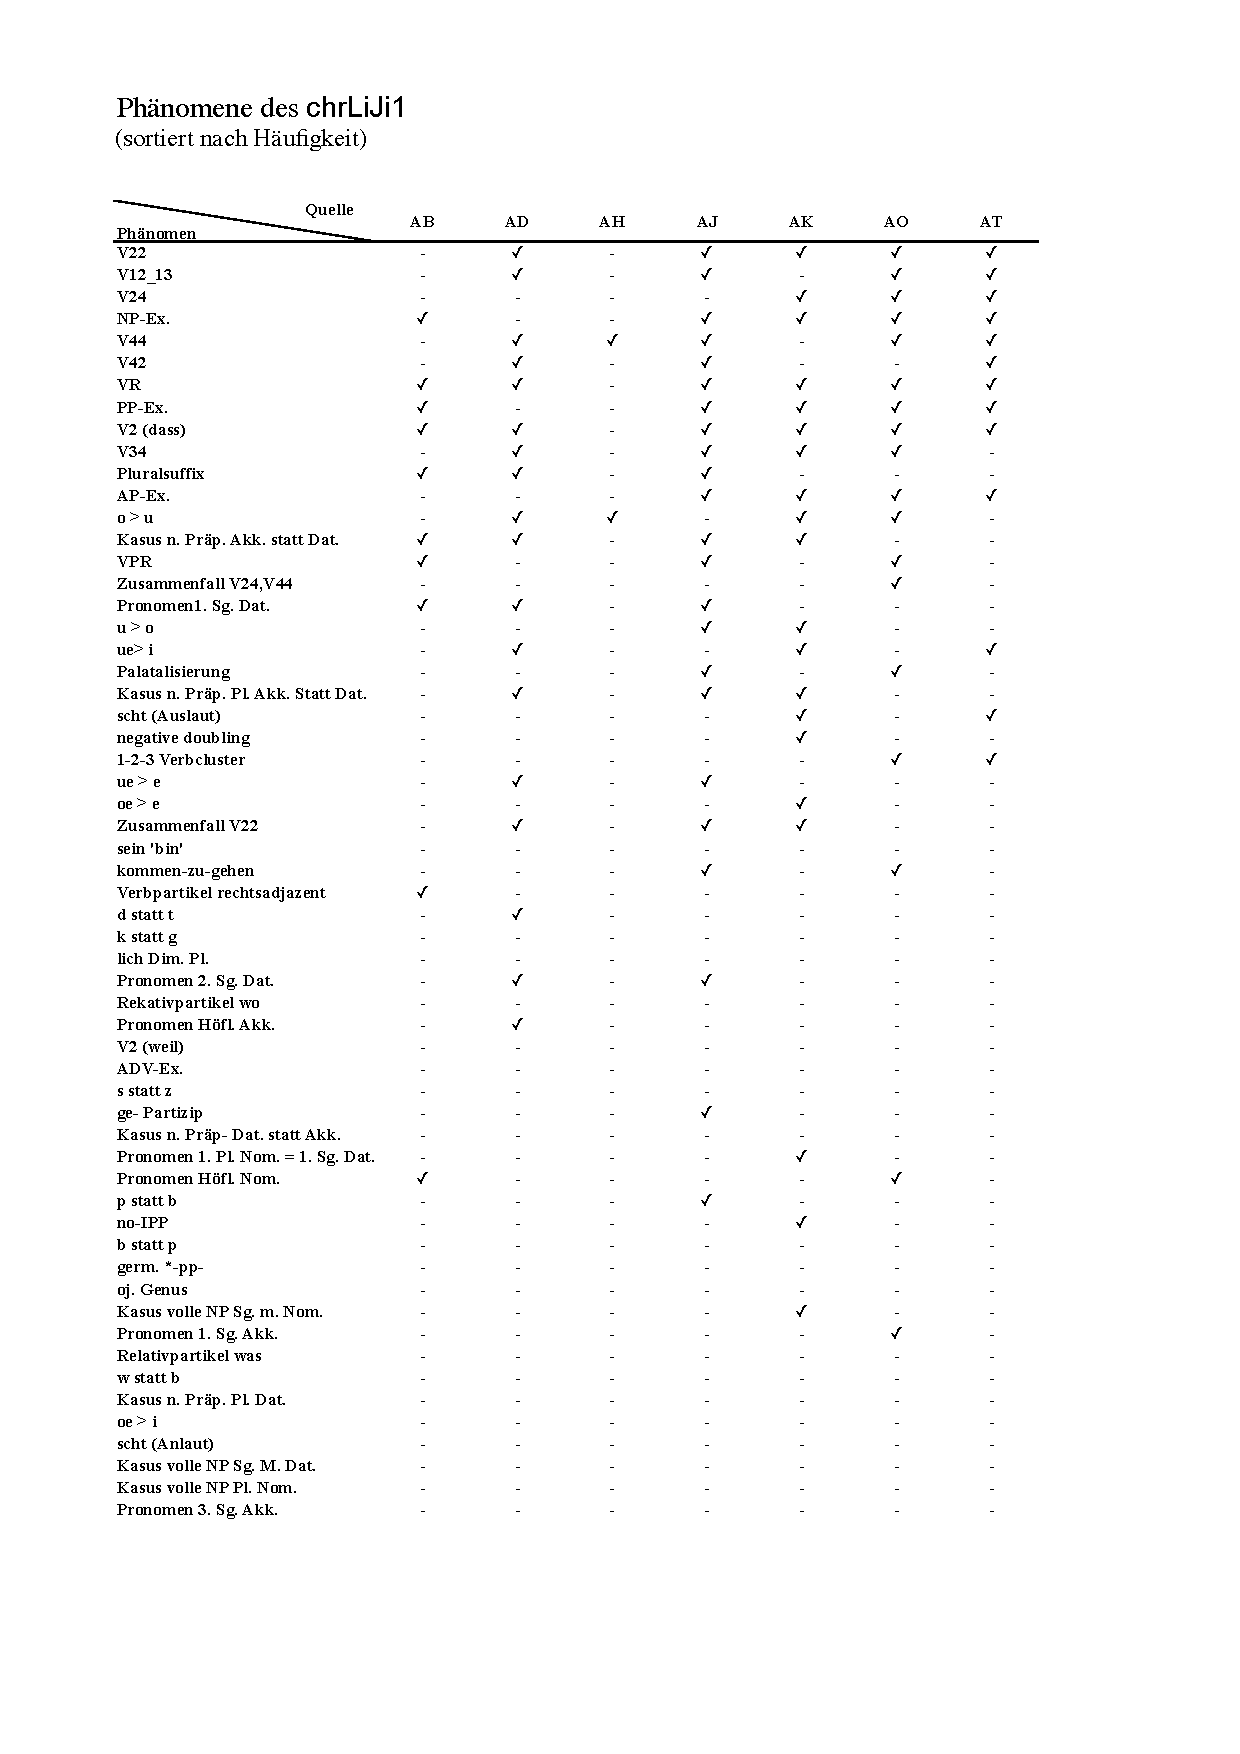
\includepdf[pages=-,pagecommand={\pagestyle{headings}}]{figures/ANHANG_ALL_END_TITEL_END.pdf} %PDF Mit Seitenzahlen PHÄNOMENTABELLE  %TT als Tabelle anführen!!?!?!?!
% %%%ende  chr\ili{LiJi1} Phänomene


%\section{Phänomentabelle \hai{jüdLiJi1}} \label{appendixphaenalljuedliji}
%%%Anfang  jüd\ili{LiJi1} Phänomene

%\begin{landscape}
\begin{longtable}{  l  l  l  l  l  l  l  l  l  l  l  }
\caption{Phänomene im \hai{jüdLiJi1}}\label{appendixphaenalljuedliji}
\\
\lsptoprule
	Phänomen  & \multicolumn{10}{c}{Quelle}\\ 
\cmidrule(lr){2-11}
	          & \rotatebox{90}{GuS1} & \rotatebox{90}{GuS5} & \rotatebox{90}{GuS10} & \rotatebox{90}{GuS15} & \rotatebox{90}{GuS23} & \rotatebox{90}{PAlsleben} & \rotatebox{90}{PBerlin1} & \rotatebox{90}{PBerlin2} & \rotatebox{90}{PBreslau} & \rotatebox{90}{PDebrecen} \\  \midrule\endfirsthead
	\midrule  Phänomen  & \multicolumn{10}{c}{Quelle}\\ \cmidrule(lr){2-11}
	          & \rotatebox{90}{GuS1} & \rotatebox{90}{GuS5} & \rotatebox{90}{GuS10} & \rotatebox{90}{GuS15} & \rotatebox{90}{GuS23} & \rotatebox{90}{PAlsleben} & \rotatebox{90}{PBerlin1} & \rotatebox{90}{PBerlin2} & \rotatebox{90}{PBreslau} & \rotatebox{90}{PDebrecen} \\  \midrule\endhead
	\lspbottomrule\endlastfoot
	V24 & \checkmark & \checkmark & \checkmark & - & \checkmark & \checkmark & \checkmark & \checkmark & \checkmark & \checkmark \\ 
	V44 & \checkmark & - & - & - & \checkmark & \checkmark & - & \checkmark & \checkmark & \checkmark \\ 
	V24,V44 & \checkmark & - & - & - & \checkmark & \checkmark & - & \checkmark & \checkmark & \checkmark \\ 
	V42 & \checkmark & - & \checkmark & - & - & \checkmark & \checkmark & \checkmark & \checkmark & - \\ 
	V22 & \checkmark & \checkmark & - & \checkmark & \checkmark & \checkmark & \checkmark & \checkmark & \checkmark & - \\ 
	\isi{Zusammenfall} V22 & \checkmark & \checkmark & - & \checkmark & \checkmark & \checkmark & \checkmark & \checkmark & \checkmark & - \\ 
	V34 & \checkmark & \checkmark & \checkmark & - & \checkmark & \checkmark & - & \checkmark & \checkmark & \checkmark \\ 
	V12\_13 & \checkmark & \checkmark & \checkmark & \checkmark & \checkmark & \checkmark & - & \checkmark & \checkmark & \checkmark \\ 
	o > u & \checkmark & \checkmark & \checkmark & - & \checkmark & \checkmark & \checkmark & - & \checkmark & - \\ 
	u > o & \checkmark & \checkmark & \checkmark & - & \checkmark & \checkmark & \checkmark & - & \checkmark & - \\ 
	\isi{Palatalisierung} & \checkmark & - & - & - & \checkmark & \checkmark & - & \checkmark & - & \checkmark \\ 
	ue > i & - & - & \checkmark & - & \checkmark & \checkmark & \checkmark & - & \checkmark & \checkmark \\ 
	ue > e & \checkmark & - & - & - & \checkmark & \checkmark & - & \checkmark & \checkmark & - \\ 
	oe > e & - & \checkmark & - & \checkmark & - & \checkmark & - & - & - & \checkmark \\ 
	oe > i & \checkmark & - & - & \checkmark & - & - & - & - & - & - \\ 
	scht (\isi{Auslaut}) & - & \checkmark & - & - & \checkmark & \checkmark & \checkmark & \checkmark & - & - \\ 
	scht (\isi{Anlaut}) & - & \checkmark & - & - & \checkmark & \checkmark & \checkmark & \checkmark & - & - \\ 
	<s> für <z> & - & - & \checkmark & - & \checkmark & \checkmark & - & \checkmark & - & - \\ 
	d statt t & - & - & - & - & - & - & - & - & - & - \\ 
	p statt b & - & - & - & - & - & - & \checkmark & \checkmark & - & - \\ 
	b statt p & - & - & - & - & - & - & - & - & - & - \\ 
	k statt g & - & - & - & - & - & - & - & - & - & \checkmark \\ 
	germ. *-pp- & \checkmark & \checkmark & \checkmark & \checkmark & \checkmark & - & \checkmark & \checkmark & - & - \\ 
	w statt b & - & - & - & - & - & \checkmark & - & - & - & - \\ 
	lich Dim. Pl. & - & - & - & - & - & - & - & - & - & \checkmark \\ 
	ge- \isi{Partizip} & \checkmark & \checkmark & - & \checkmark & - & - & \checkmark & \checkmark & - & - \\ 
	oj. \isi{Genus} & - & - & - & - & \checkmark & - & - & - & - & - \\ 
	Kasus NP Sg.m. Nom. & - & - & - & - & - & - & - & - & - & - \\ 
	Kasus NP Sg.m.Dat. & - & - & - & - & - & - & - & - & - & - \\ 
	Kasus NP Pl.Nom. & - & - & - & - & - & - & - & - & - & - \\ 
	Kasus n. Präp. Akk. statt Dat. & \checkmark & \checkmark & \checkmark & \checkmark & - & - & \checkmark & \checkmark & \checkmark & - \\ 
	Kasus n. Präp. Dat statt Akk. & - & - & - & - & - & - & - & - & - & - \\ 
	Kasus n. Präp. Akk. Pl. & - & - & \checkmark & - & \checkmark & - & \checkmark & - & - & - \\ 
	Kasus n. Präp. Pl. Dat. & - & - & - & - & - & - & - & - & - & - \\ 
	\isi{Pronomen} 1.Sg.Dat. & \checkmark & \checkmark & \checkmark & \checkmark & \checkmark & \checkmark & - & - & \checkmark & - \\ 
	\isi{Pronomen} 1.Sg.Akk. & - & - & - & - & - & - & - & - & - & - \\ 
	\isi{Pronomen} 2.Sg.Dat. & - & - & \checkmark & - & - & - & - & - & \checkmark & - \\ 
	\isi{Pronomen} 3.Sg.Akk. & - & - & - & - & - & - & - & - & - & - \\ 
	\isi{Pronomen} 1.Pl.Nom=1.Sg.Dat. & \checkmark & \checkmark & - & - & - & - & - & \checkmark & - & - \\ 
	\isi{Pronomen} Höfl. Nom. & - & - & \checkmark & - & \checkmark & - & \checkmark & - & - & - \\ 
	\isi{Pronomen} Höfl. Dat. & - & - & - & - & - & \checkmark & - & - & - & - \\ 
	\isi{Pluralsuffix} & \checkmark & \checkmark & \checkmark & \checkmark & \checkmark & - & \checkmark & \checkmark & - & - \\ 
	sein 'bin' & \checkmark & - & - & - & - & - & \checkmark & \checkmark & - & - \\ 
	kommen-zu-gehen & - & \checkmark & - & - & - & - & - & - & - & - \\ 
	\isi{negative doubling} & - & - & - & - & \checkmark & - & - & - & \checkmark & - \\ 
	no-IPP & - & \checkmark & - & \checkmark & \checkmark & \checkmark & \checkmark & - & \checkmark & \checkmark \\ 
	1-2-3 \isi{Verbcluster} & - & - & \checkmark & - & - & \checkmark & \checkmark & \checkmark & - & - \\ 
	VR & \checkmark & \checkmark & \checkmark & \checkmark & \checkmark & \checkmark & \checkmark & \checkmark & \checkmark & - \\ 
	\isi{Relativpartikel} wo & - & - & - & - & - & - & - & - & - & - \\ 
	\isi{Relativpartikel} was & \checkmark & \checkmark & \checkmark & \checkmark & \checkmark & \checkmark & \checkmark & - & - & - \\ 
	VPR & \checkmark & \checkmark & - & - & - & - & \checkmark & - & \checkmark & - \\ 
	\isi{Verbpartikel} rechtsdkazent & - & - & - & - & - & - & \checkmark & \checkmark & - & - \\ 
	V2 (dass) & \checkmark & \checkmark & \checkmark & \checkmark & \checkmark & \checkmark & \checkmark & \checkmark & \checkmark & - \\ 
	V2 (weil) & \checkmark & - & - & - & - & - & - & - & \checkmark & - \\ 
	NP-Ex. & \checkmark & \checkmark & \checkmark & \checkmark & \checkmark & \checkmark & \checkmark & \checkmark & \checkmark & \checkmark \\ 
	PP-Ex. & \checkmark & \checkmark & \checkmark & \checkmark & \checkmark & \checkmark & \checkmark & \checkmark & \checkmark & - \\ 
	AP-Ex. & \checkmark & \checkmark & - & - & \checkmark & - & \checkmark & \checkmark & - & - \\ 
	Adv.-Ex. & - & - & - & - & - & - & - & - & - & - \\ 
\end{longtable}
%\end{landscape}
% 
% %PFD  jüd\ili{LiJi1} Phänomene
% %\begin{landscape}
% \thispagestyle{empty}
% \markboth{Phänomentabelle \hai{jüdLiJi1}}{Phänomentabelle \hai{jüdLiJi1}}

% 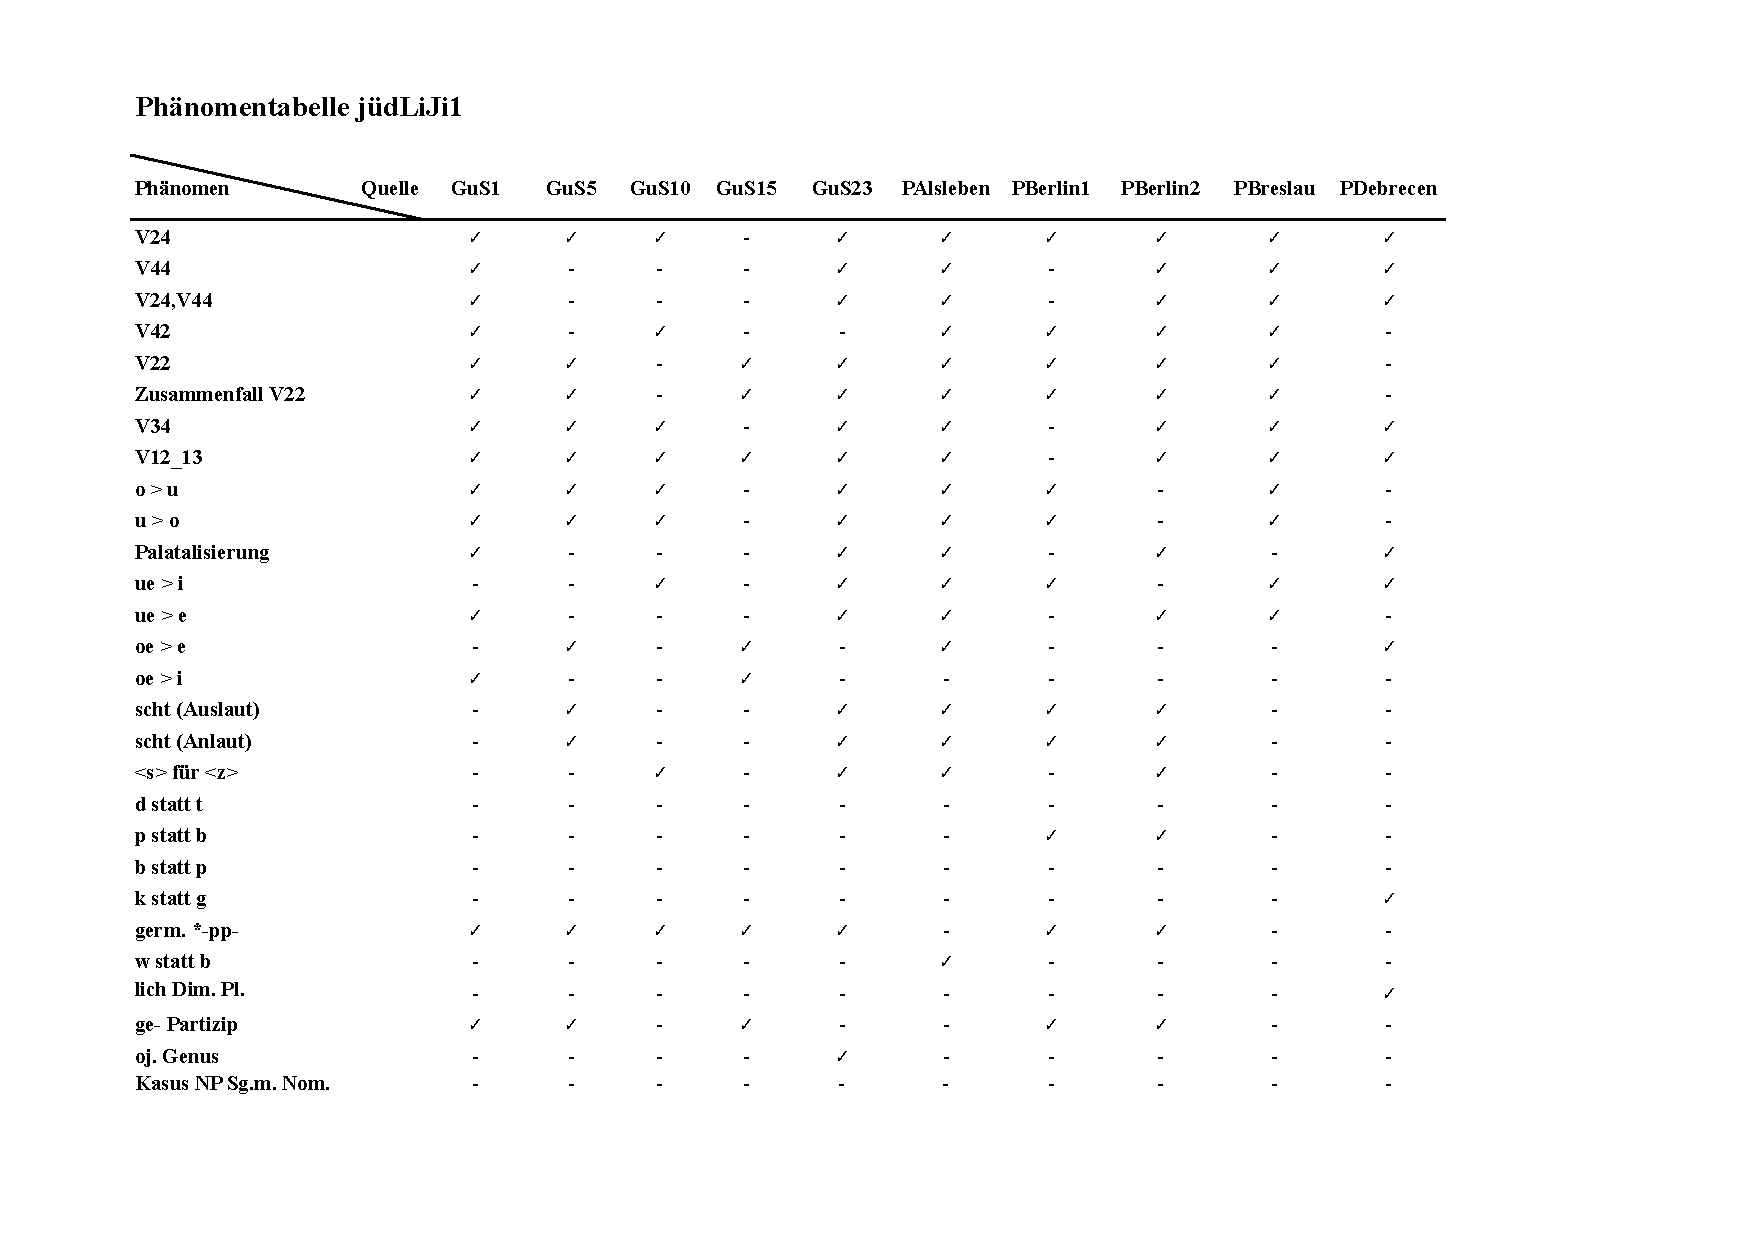
\includepdf[pages=-,pagecommand={\pagestyle{headings}},landscape=true]{figures/Anhang_juedLiJi1_ALL.pdf} 


%%%ende  jüd\ili{LiJi1} Phänomene
%%%%%%%%%%%%%%%%%%%%%%%%%%%%%%%%%%%%%%%%%%%%%%%%%%%%%%%%%%%%%%%%%%%%%%%%%%%%%%%
%%%%%%%%%%%%%%%%%%%%%%%%%%%%%%%%%%%%%%%%%%%%%%%%%%%%%%%%%%%%%%%%%%%%%%%%%%%%%%%

%\thispagestyle{empty}
%\markboth{Datengrundlage: Korpora \hai{chrLiJi1} und \hai{jüdLiJi1}}{Datengrundlage: Korpora \hai{chrLiJi1} und \hai{jüdLiJi1}	 }
%	\phantomsection \addcontentsline{toc}{section}{Datengrundlage: Korpora \hai{chrLiJi1} und \hai{jüdLiJi1}} \label{appendixkorpus}
%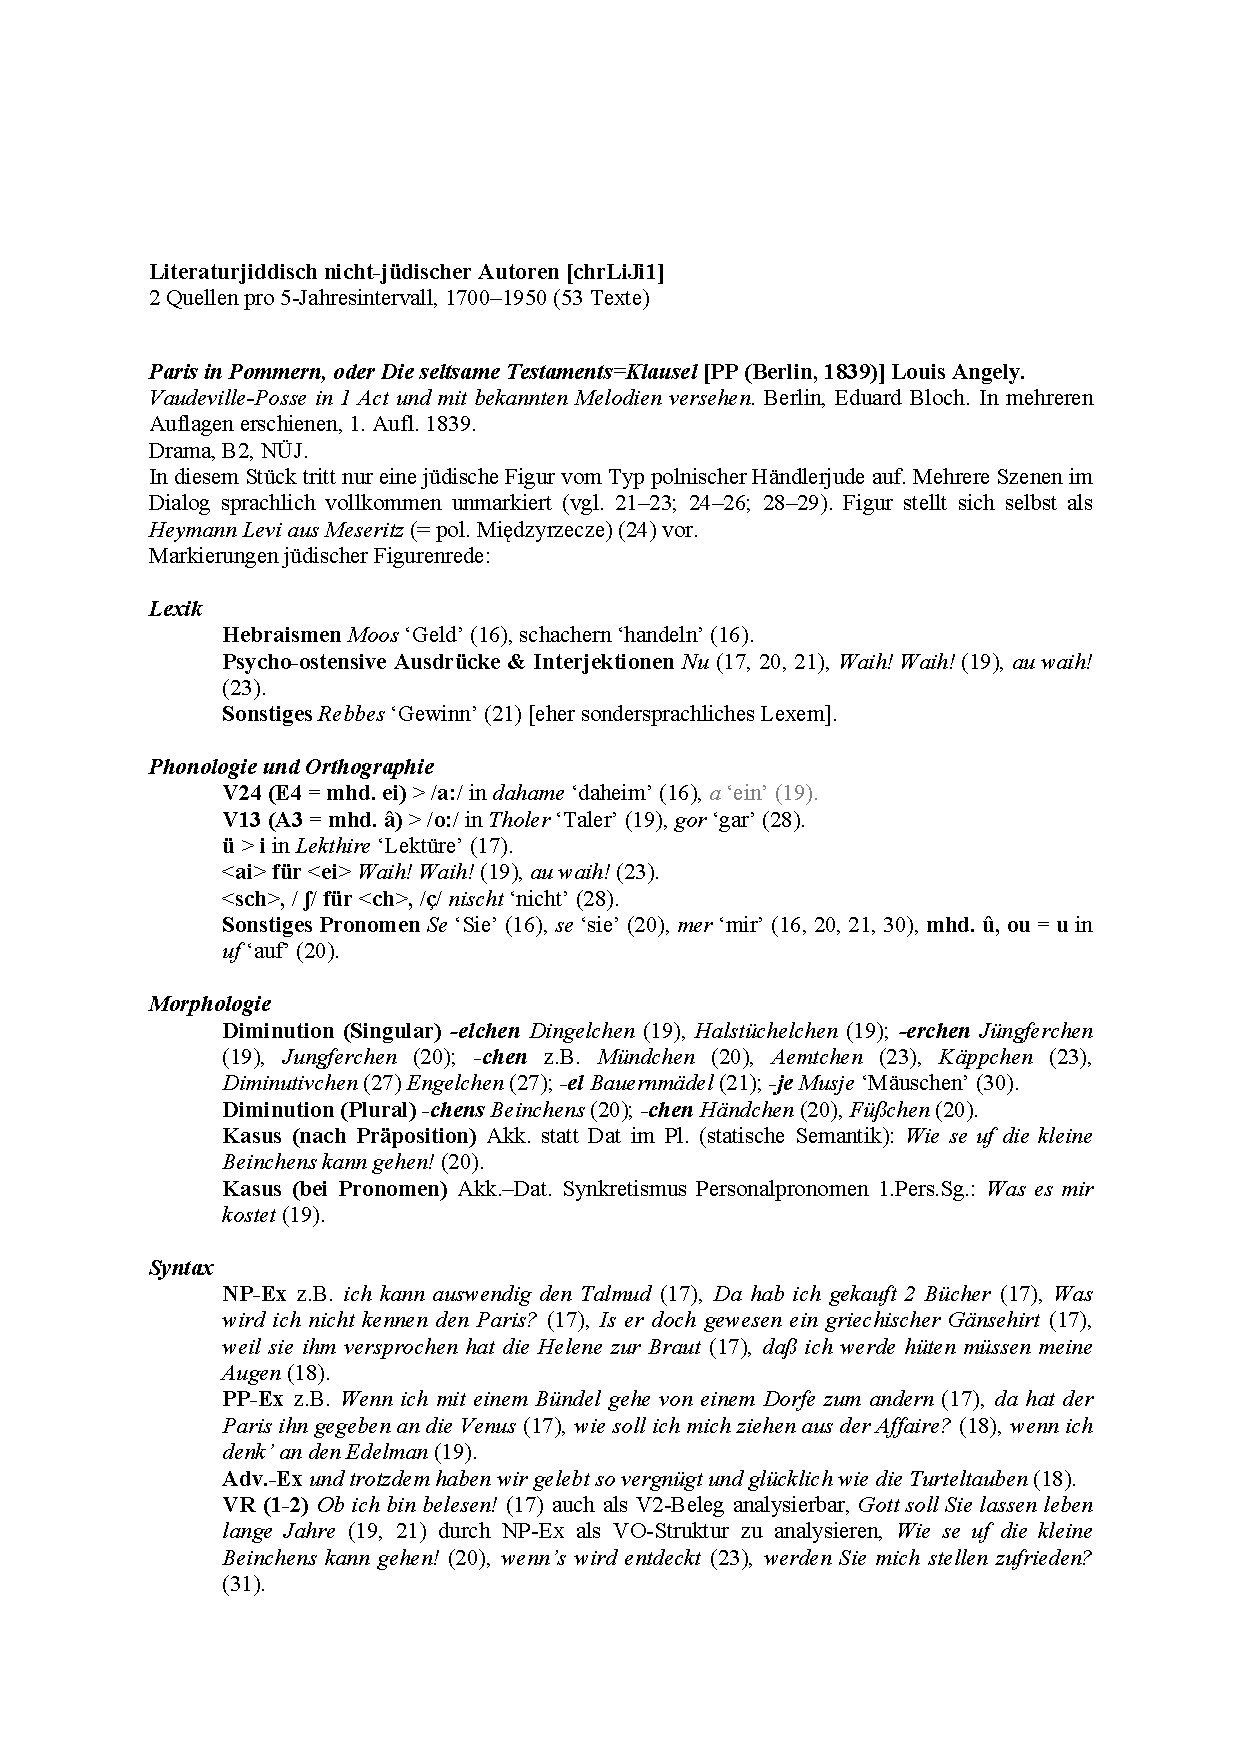
\includepdf[pages=-,pagecommand={\pagestyle{headings}}]{figures/Korpus_End_LSP.pdf} %PDF Mit 


\newpage
\thispagestyle{empty}
\markboth{Hs. 40a Ruhr. 16 Nr. 22 des Hessischen Staatsarchivs Marburg}{Hs. 40a Ruhr. 16 Nr. 22 des Marburger Staatsarchivs}\label{part_schirm}


%\phantomsection \addcontentsline{toc}{section}{Transliteration und Scan der Hs. 40a Ruhr. 16 Nr. 22 des Marburger Staatsarchivs}\label{appendixschirm}%\addtocounter{page}{1} 
\includepdf[pages=-,pagecommand={\pagestyle{headings}}]{figures/Anhang_Schirm.pdf}\label{appendixschirm}

\normalsize